\RequirePackage{fix-cm}
\documentclass[smallextended,twocolumn,natbib]{svjour3}
\usepackage[colorlinks,citecolor=blue,linkcolor=blue]{hyperref}
%\usepackage[style=authoryear,natbib=true]{biblatex}
%\addbibresource{egbib.bib}
\bibliographystyle{spbasic}
\smartqed  % flush right qed marks, e.g. at end of proof
%
\makeatletter
\def\cl@chapter{\cl@chapter \@elt {theorem}}%bug in class
\def\cl@chapter{\@elt {theorem}}
% Patch case where name and year are separated by aysep
\patchcmd{\NAT@citex}
  {\@citea\NAT@hyper@{%
     \NAT@nmfmt{\NAT@nm}%
     \hyper@natlinkbreak{\NAT@aysep\NAT@spacechar}{\@citeb\@extra@b@citeb}%
     \NAT@date}}
  {\@citea\NAT@nmfmt{\NAT@nm}%
   \NAT@aysep\NAT@spacechar\NAT@hyper@{\NAT@date}}{}{}

% Patch case where name and year are separated by opening bracket
\patchcmd{\NAT@citex}
  {\@citea\NAT@hyper@{%
     \NAT@nmfmt{\NAT@nm}%
     \hyper@natlinkbreak{\NAT@spacechar\NAT@@open\if*#1*\else#1\NAT@spacechar\fi}%
       {\@citeb\@extra@b@citeb}%
     \NAT@date}}
  {\@citea\NAT@nmfmt{\NAT@nm}%
   \NAT@spacechar\NAT@@open\if*#1*\else#1\NAT@spacechar\fi\NAT@hyper@{\NAT@date}}
  {}{}
\makeatother


%\documentclass[lettersize,journal]{IEEEtran}

%% The amssymb package provides various useful mathematical symbols
\usepackage[dvipsnames]{xcolor} 
\usepackage{graphicx}
\usepackage{amssymb}
\usepackage{amsmath}
\usepackage{array}
\usepackage{lineno}
\usepackage{comment}
\usepackage{multirow}
\usepackage{cite}
\usepackage{subcaption}
\usepackage{threeparttable,booktabs}
%\usepackage[numbers,sort&compress]{natbib}
\usepackage{etoolbox}
\renewcommand{\tablename}{Table}
%\usepackage[justification=centering]{caption} % Figures caption
\captionsetup{labelsep = period} 
\renewcommand{\figurename}{Fig.} % Fig.2 (rather than Figure 2)
\usepackage[export]{adjustbox}
%\usepackage{caption, subcaption}
\usepackage{diagbox}
\usepackage{totcount}
\usepackage{overpic}
\newtotcounter{citenum}
\usepackage{pifont}
\usepackage{makecell}
\usepackage{totcount}
\captionsetup{%
    justification=Justified,%
}

% Include other packages here, before hyperref.

\usepackage{cleveref}
\definecolor{applegreen}{rgb}{0.0, 0.5, 0.0}
\definecolor{cadmiumred}{rgb}{0.89, 0.0, 0.13}

\definecolor{babyblue}{HTML}{7EA6E0}
\definecolor{fadedred}{HTML}{EA6B66}
\definecolor{pastelorange}{HTML}{FFB570}
\definecolor{pastelteal}{HTML}{67AB9F}
\definecolor{pastelpurple}{HTML}{B5739D}




\newcommand\tstrut{\rule{0pt}{2.4ex}}
\newcommand\bstrut{\rule[-1.0ex]{0pt}{0pt}}

\newtotcounter{citnum} %From the package documentation
\def\oldbibitem{} \let\oldbibitem=\bibitem
\def\bibitem{\stepcounter{citnum}\oldbibitem}


\newcommand*{\upSmallFrown}{\mathbin{\raisebox{0.9ex}{$\smallfrown$}}}


\usepackage{balance}



\begin{document}


\title{A Hitchhiker's Guide to Action Understanding: Advances, Challenges, and Outlooks}
% Points in Time
% Or The Test of Time
% Or... Past Due: 
% Or... The past, present and future of time in action understanding

%\author{Alexandros Stergiou$^1$, Ronald Poppe$^2$
%\thanks{\looseness-1 $^1$Alexandros Stergiou is with the Faculty of Electrical Engineering, Mathematics and Computer Science at the University of Twente, Drienerlolaan 5, 7522 NB Enschede, The Netherlands (e-mail:a.g.stergiou@utwente.nl)\\ 
%\indent
%$^2$Ronald Poppe is with the Department of Information and Computing Sciences at Utrecht University, Princetonplein 5, 3584 CC Utrecht, The Netherlands (e-mail: r.w.poppe@uu.nl)}}
%\markboth{Journal of \LaTeX\ Class Files,~Vol.~18, No.~9, September~2020}%
%{How to Use the IEEEtran \LaTeX \ Templates}


\author{Alexandros Stergiou \and Ronald Poppe}
\institute{A. Stergiou \at Faculty of Electrical Engineering, Mathematics and Computer Science at the University of Twente, Drienerlolaan 5, 7522 NB Enschede, The Netherlands   
\and
R.Poppe \at Department of Information and Computing Sciences at Utrecht University, Princetonplein 5, 3584 CC Utrecht, The Netherlands
}
%\date{Received: date / Accepted: date}
% The correct dates will be entered by the editor


\maketitle

\begin{abstract}
%% Text of abstract
We have witnessed impressive advances in action understanding research, both in terms of accuracy, and in the diversification of tasks. We are increasingly capable of extracting more meaningful information from action videos. Powered by datasets of expanded sizes and the upscaled computation availability, current systems can provide fine- and coarse-grained descriptions of video scenes, extract segments corresponding to queries, synthesize unobserved parts of the video, and predict the context of videos. This survey provides a comprehensive review of recent advances in uni-and-multi-modal action understanding. We focus on the prevalent challenges, overview widely adopted datasets, and survey seminal works. We focus on how temporal information is used, distinguishing broadly between action classification, prediction, and forecasting. This division allows us to identify specific challenges. Finally, we provide an outward look into future directions to address current shortcomings.

\end{abstract}

%\begin{IEEEkeywords}
%Class, IEEEtran, \LaTeX, paper, style, template, typesetting.
%\end{IEEEkeywords}

\keywords{Action Understanding \and t2 \and t3}

%% main text

\section{Introduction}


% Preface paragraph
Rapid technological advancements have integrated into multiple aspects of our everyday life. Digital processing of information has enabled greater levels of automation enhancing our quality of life. These advancements allow us to capture, share, and consume footage of our or other's everyday experiences. The definition of algorithms able to \emph{understand} these experiences and the actions performed has been of particular interest to the computer vision community since its early days. 



% Action understanding in cognitive science 
In neuroscience, \emph{action understanding} has been explored across several distinct psychological processes \citep{thompson2019conceptualizing}. Aspects include; \emph{The capacity to understand the action being performed}. This defines the capability to differentiate between analogous actions \citep{gallese1996action,jeannerod1994representing} and the conceptualization of how an action is performed \citep{spunt2011identifying}. \emph{Determining the goal of the action}. Works \citep{calvo2005action,kohler2002hearing,rizzolatti2001neurophysiological} have studied action understanding in relation to the immediate goals of actions. This includes both motor functions for executing an action and sensory perception of actions performed by others. \emph{Determining the actor's intention}. In contrast to goals that can be understood immediately after an action's completion, intentions relate to high-level motivations for performing an action \citep{kilner2011more}. Such intentions have been defined by the sequential grouping of individual actions \citep{fogassi2005parietal} and their abstract associated target \citep{uithol2011understanding}.

\begin{figure*}[t]
    \centering
    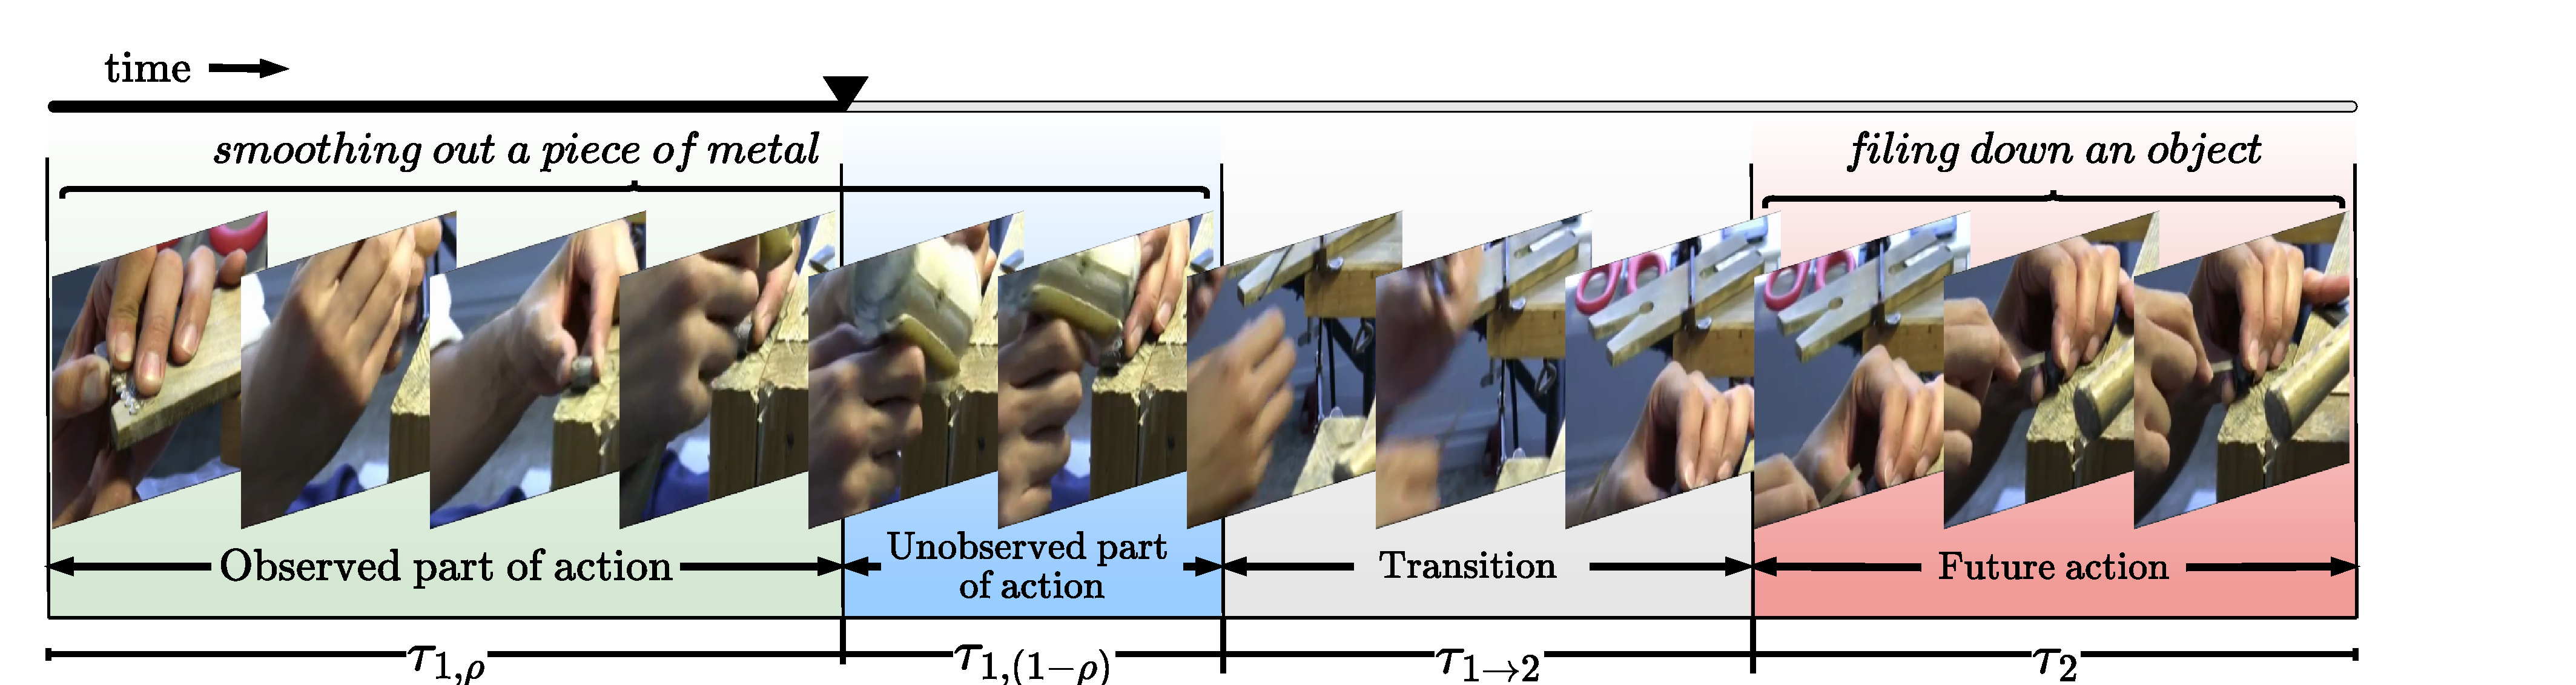
\includegraphics[width=\linewidth,trim={1cm 0 6cm 0},clip]{figs/action_understanding_tasks.pdf}
    \caption{\textbf{Action understanding tasks}. The progress of the video is shown by the top bar. Given an action that is currently being performed, and with duration $\tau_1$, only $\tau_{1,\rho}<\tau_1 $ part of the action is currently observable. After a short transition period $0\leq\tau_{1 \rightarrow 2}$ another action is performed with duration $\tau_2$. \textbf{Action recognition} tasks are based on full observations of the action at $\tau_1$. \textbf{Ongoing action prediction} uses only part $\tau_{1,\rho}$ of ongoing action. \textbf{Action forecasting} uses current action at $\tau_1$ to predict future actions. Example selected from \citep{wang2019vatex}.} 
    \label{fig:tasks}
\end{figure*}

% Temporal scopes
Inspired by the human cognition aspects of action understanding, we define three broad \emph{temporal scopes} and group seminal machine vision action understanding methods accordingly. We visualize the evolution of a video in~\Cref{fig:tasks} when an action is currently being performed and a subsequent action will follow next. We group tasks that require the first action to be \emph{observed in full} as \textbf{recognition} tasks, which infer information such as action categories or high-level semantics. Instead, if the prediction about ongoing actions is made from the action being only \emph{partially observed}, we group these tasks as \textbf{prediction} tasks. The final temporal focus of \textbf{forecasting} tasks is to use reasoning from the currently observed action for the future action \emph{not yet observed}. For each temporal scope, we discuss previous surveys that provide condensed overviews of advancements across different tasks and application domains.

\noindent
\textbf{Recognition}. Early works on action recognition have primarily focused on overviewing motion modeling. \citet{aggarwal1994articulated} defined a taxonomy of motions based on rigidness with a subsequent overview \citep{aggarwal1998nonrigid} of further subdivisions based on prior knowledge of the objects' shape. \citet{cedras1995motion} and later \citet{moeslund2001survey} discussed temporal modeling approaches in the context of classification and tracking. As overviewed by \citet{buxton2003learning} tracking approaches have also been used in more complex tasks such as behavior analysis or non-verbal human interactions. A division in modeling and estimation of human motions was later discussed by \citet{poppe2007vision}. 
% Classification surveys
Later overviews included more explicit scopes such as action classification, and localization \citep{weinland2011survey}, behavior understanding \citep{chaaraoui2012review}, or surveillance applications \citep{vishwakarma2013survey}. They explored task-specific advancements on more semantically complex topics, primarily relating to classification. \citet{turaga2008machine} and \citet{poppe2010survey} both discussed approaches addressing atomic actions and group activities. \citet{herath2017going} provided an initial summary of learned-feature approaches for action recognition. Later surveys overviewed the adoption and adaptation of deep learning approaches for topics such as; depth-based motion recognition \citep{wang2018rgb}, activity recognition \citep{beddiar2020vision}, human-human interactions \citep{stergiou2019analyzing}, and pose estimation \citep{zheng2020deep}. \citet{sun2022human} reviewed approaches across multiple modalities combining motion features, audio, and vision. More recently, \citet{selva2023video} overviewed attention-based approaches for video tasks while \citet{schiappa2023self} focused on self-supervised approaches.

\noindent
\textbf{Prediction}. The advancements in the recognition of actions in videos have recently enabled the definition of more challenging predictive tasks from partial observations. \citet{rasouli2020deep} discussed four main domains of predictive models including video, action, trajectory, and motion prediction. \citet{kong2022human} described recent advancements for action recognition and prediction focusing on their applications to domains such as robot vision, surveillance, and driver behavior prediction. The surveys of \citet{dhiman2019review} and later \citet{ramachandra2020survey} overviewed predictive methods for anomaly detection tasks.




\noindent
\textbf{Forecasting}. Similarly, forecasting tasks have more recently been at the forefront of research. \citet{rodin2021predicting} discussed prevalent approaches for future action anticipation in egocentric videos. \citet{zhong2023survey} overviewed both short and long-term approaches for predicting actions into the future. \citet{hu2022online} provided a review of both online and anticipation approaches. More recently, \citet{plizzari2024outlook} discussed challenges in egocentric videos and provided future direction outlooks for multiple scopes including forecasting tasks.


%Considering the vastness of tasks that study changes in the visual information across time, an answer to the question \emph{where does one start from?} may be less easy to define.
% Motion modeling



 
  
% Addressing multiple aspects of action understanding
Despite providing extensive overviews, prior surveys focus on specific aspects of action understanding. As summarized in \Cref{tab:surveys}, an overview over critical works of the past decades across multiple aspects of action understanding is missing from the current literature. 


% TODO paragraph on survey focus and structure
In this survey we address the diversity of action understanding tasks by their use of the temporal dimension. We overview the general methods for modeling actions in videos over the years in~\ref{sec:modeling}. We discuss datasets and benchmarks used by prior works in~\Cref{sec:datasets}. Following the defined action understanding tasks categories, we first distinguish tasks that require actions to be observed in their entirety to infer their semantics in~\Cref{sec:recognition}. Tasks that aim to predict ongoing actions in which only parts of the action are observed are overviewed in~\Cref{sec:prediction}. We discuss tasks and approaches that aim to anticipate what will happen next in~\Cref{sec:forecasting}. For each of these directions we outline main challenges and provide our insights as to what the future of action understanding may look like in~\Cref{sec:outlook}. We conclude with a summary of this survey's findings and general thoughts in~\Cref{sec:discussion}.


\begin{table*}[t]
    \centering
    \caption{\textbf{Action understanding surveys through the years}. Columns highlight the temporal scope of surveys; with works on either recognition (Rec.), prediction (Pred.), or anticipation (Ant.). The reported broad objectives that surveys overview include multi-modality (MM), self-supervision (Self-Sup.), and multi-view (MV). The two tasks of interest tracked among surveys are human interactions (HI) to either objects or other humans, and long video understanding (LVU). Scopes/objectives/tasks addressed partially by surveys are denoted with (partial) and the main focus is denoted with \ding{52}.}
    \resizebox{\textwidth}{!}{
    \begin{tabular}{l c c c c c l c c c l c c}
    \toprule
    \multirow{2}{*}{Author(s)} & 
    \multirow{2}{*}{Year} &
    \multirow{2}{*}{\#Papers} & \multicolumn{3}{c}{Temporal Scope} & $\;$ & \multicolumn{3}{c}{Objectives} & $\;$ & \multicolumn{2}{c}{Tasks} \bstrut\\ \cline{4-6}\cline{8-10}\cline{12-13}
    & & &
    Rec. & Pred. & Ant. & $\;$ & MM & Self-Sup. & MV & $\;$ & HI & LVU  \tstrut\\
    \midrule
    \citet{aggarwal1994articulated} & 1994 & 
    69 &  
    (partially) & 
      & 
      && 
      & 
      & 
      && 
      & \\
    \citet{cedras1995motion} & 1995 &
    76 &  
      (partially) & 
      & 
      && 
      & 
      & 
      && 
      & \\
    \citet{aggarwal1998nonrigid} & 1998 & 
    104 &  
      (partially) & 
      & 
      && 
      & 
      & 
      && 
      & \\ 
    \citet{aggarwal1999human} & 1999 & 
    51 &  
      (partially) & 
      & 
      && 
      & 
      & 
      && 
      & \\
    \citet{moeslund2001survey} & 2001 &
    155 &  
      (partially) & 
      & 
      && 
      & 
      & 
      && 
      & \\
    \citet{buxton2003learning} & 2003 & 
    88 &  
      (partially) & 
      & 
      && 
      & 
      &
      &&
      \ding{52}
      & \\
    \citet{moeslund2006survey} & 2006 & 
    424 &  
      \ding{52} & 
      & 
      && 
      (partially) & 
      & 
      && 
      & \\
    \citet{yilmaz2006object} & 2006 &
    160 &  
      (partially) & 
      (partially) & 
      && 
      & 
      & 
      && 
      (partially) &
      \\
    \citet{poppe2007vision} & 2007 & 
    125 &  
      \ding{52} & 
      & 
      && 
      (partially) & 
      & 
      && 
      & \\
    \citet{turaga2008machine} & 2008 &
    144 &  
      \ding{52} & 
      & 
      && 
      (partially) & 
      & 
      && 
      \ding{52} &
      \\
    \citet{poppe2010survey} & 2010 & 
    180 &  
      \ding{52} & 
      & 
      && 
      & 
      & 
      && 
      & \\
    \citet{weinland2011survey} & 2011 & 
    153 &  
      \ding{52} & 
      & 
      && 
      (partially) & 
      & 
      (partially) &&
      \ding{52} &\\
    \citet{chaaraoui2012review} & 2012 &
    123 &  
      \ding{52} & 
      & 
      && 
      (partially) & 
      & 
      \ding{52} &&
      \ding{52} &\\
    \citet{metaxas2013review} & 2013 &
    188 &  
      & 
      & 
      && 
      & 
      & 
      (partially) && 
      \ding{52} & \\
    \citet{vishwakarma2013survey} & 2013 &
    231 &  
      \ding{52} & 
      & 
      && 
      (partially) & 
      & 
      && 
      & \\
    \citet{herath2017going} & 2017 & 
    161 &  
      \ding{52} & 
      & 
      && 
      & 
      & 
      && 
      & \\
    \citet{wang2018rgb} & 2018 & 
    182 &  
      \ding{52} & 
      (partially) & 
      && 
      (partially) & 
      & 
      (partially) && 
      (partially) & \\
    \citet{dhiman2019review} & 2019 & 
    208 &  
      & 
      & 
      \ding{52} && 
      (partially) & 
      & 
      &&
      (partially) & \\
    \citet{hussain2019different} & 2019 & 
    141 &  
      \ding{52} & 
       & 
      && 
      \ding{52} & 
      & 
      (partially) && 
      \ding{52} & \\
    \citet{stergiou2019analyzing} & 2019 & 
    178 &  
      \ding{52} & 
      & 
      && 
      & 
      & 
      && 
      \ding{52} & \\
    \citet{yao2019review} & 2019 &
    106 &  
      \ding{52} & 
      & 
      && 
      & 
      & 
      && 
      & \\
    \citet{zhang2019comprehensive} & 2019 &
    127 &  
      \ding{52} & 
      & 
      && 
      & 
      & 
      && 
      & \\
    \citet{beddiar2020vision} & 2020 & 
    237 &  
      \ding{52} & 
      & 
      (partially) && 
      & 
      & 
      (partially) && 
      \ding{52} & 
      \\
      \citet{ramachandra2020survey} & 2020 &
    109 &  
      & 
      \ding{52} & 
      && 
      & 
      & 
      && 
      & \\
    \citet{zheng2020deep}& 2020 & 
    317 &  
      & 
      & 
      && 
      \ding{52} & 
      & 
      && 
      & \\
    \citet{rasouli2020deep} & 2020 &
    333 &  
      & 
      \ding{52} & 
      && 
      & 
      & 
      && 
      & \\
    \citet{pareek2021survey} & 2021 & 
    218 &  
      \ding{52} & 
      & 
      && 
      (partially) & 
      & 
      && 
      & \\
    \citet{rodin2021predicting}& 2021 & 
    156 &  
      & 
      & 
      \ding{52} && 
      (partially) & 
      & 
      \ding{52} && 
      & 
      \ding{52} \\
    \citet{song2021human} &
    2021 &
    157 &  
      \ding{52} & 
      & 
      && 
      & 
      & 
      && 
      & \\
    \citet{sun2022human} & 2022 & 
    503 &  
      \ding{52} & 
      & 
      && 
      (partially) & 
      \ding{52} & 
      && 
      & \\
    \citet{kong2022human} & 2022 & 
    337 &  
      \ding{52} & 
      (partially) & 
      && 
      & 
      & 
      \ding{52} && 
      (partially) & \\ 
    \citet{hu2022online} & 2022 & 
    168 &  
      \ding{52} & 
      & 
      \ding{52} && 
      & 
      & 
      && 
      \ding{52} & 
      (partially) \\
    \citet{oprea2022review} & 2022 & 
    211 &  
      \ding{52} & 
      \ding{52} & 
      && 
      & 
      & 
      && 
      & \\
    \citet{schiappa2023self} & 2023 &
    216 &  
      \ding{52} & 
      & 
      && 
      & 
      \ding{52} & 
      \ding{52} && 
      & 
      \ding{52}\\
    \citet{selva2023video} & 2023 &
    209 &  
      \ding{52} & 
      & 
      && 
      & 
      & 
      && 
      & \\
    \citet{wang2023temporal} & 2023 & 229 & \ding{52} & 
      & 
      && 
      (partially) & 
      & 
      (partially) && 
      & \\
    \citet{zhong2023survey} & 2023 & 
    207 &
      & 
      & 
      \ding{52} && 
      \ding{52} & 
      \ding{52} & 
      \ding{52} && 
      & 
      \ding{52} \\  
    \citet{ding2023temporal} & 2023 & 
    168 &  
      \ding{52} & 
      & 
      && 
      & 
      & 
      \ding{52} && 
      & 
      (partially) \\ 
    \citet{plizzari2024outlook} & 2024&
    367 &
      \ding{52} & 
      & 
      \ding{52} && 
      \ding{52} & 
      & 
      \ding{52} && 
      \ding{52} & 
      \ding{52}  \\
    \midrule
    Stergiou and Poppe (\textbf{this survey}) & 2024 & \textbf{\total{citnum}} & 
    \ding{52} & 
    \ding{52} & 
    \ding{52} && 
    \ding{52} & 
    \ding{52} & 
    \ding{52} && 
    \ding{52} & 
    \ding{52} \\
    \end{tabular}
    }
    \label{tab:surveys}
\end{table*}



\section{Modeling actions in videos}
\label{sec:modeling}

% section intro
Video is composed of spatial information that relates to visual aspects of objects, background information, or the visual context of scenes. It also includes temporal information corresponding to changes of these visual aspects over time. In this section we overview two general approaches for encoding space-time information from videos without explicitly relating them to tasks. The first set of approaches discussed in~\Cref{sec:modeling::separate} model spatial features and temporal information separately. The second create joint spatio-temporal representations that are overviewed in~\Cref{sec:modeling::joint}.


\subsection{Separating visual and temporal information}
\label{sec:modeling::separate}

\noindent
\textbf{Tracking and template matching}. Early works \citep{bobick2001recognition} have considered template-matching approaches for determining spatial and temporal locations where motions occur. Template-based methods have also been explored over local patches \citep{shechtman2005space}, through correlation filters \citep{rodriguez2008action}, or based on voxel similarity \citep{ke2007spatio}. A different direction of research has considered the discovery of temporal patterns by tracking visual features over time \citep{cipolla1990dynamic,isard1998condensation,rohr1994towards}. 


\noindent
\textbf{Local descriptors}. A key characteristic of actions is appearance changes over time. Multiple methods have proposed approaches to associate changes in local features with actions. Mikolajczyk and Uemura \citep{mikolajczyk2008action} clustered local features to tree representations and related them to action categories. Similarly, pose-based primitives \citep{thurau2008pose}, temporal bins \citep{nowozin2007discriminative}, pictorial structures \citep{tran2012part}, and graphical structures of the actions \citep{ni2014multiple} have been used with local descriptor features. Other approaches \citep{gupta2009observing,yao2010modeling} cast action recognition as a structural connectivity task by recognizing parts of objects and understanding actions by pose.
Following methods have also extended this to individual regions \citep{ikizler2010object}, poselet clusters \citep{pishchulin2013strong}, decision trees \citep{rahmani2014real}, and covariance matrices \citep{kviatkovsky2014online}.  


% CNN-based action recognition
\noindent
\textbf{Spatial convolutions}. CNNs have become widely used feature extractors for a variety of vision tasks. An initial effort \citep{karpathy2014large} to fuse temporal information with CNN's static features included the combination of frame embeddings either in the first few layers or final layers of the architecture. Others explored the factorization of frame embeddings \citep{sun2015human}, frame ranking \citep{fernando2015modeling}, pooling \citep{fernando2016rank}, salient region focus \citep{girdhar2017attentional, zong2021motion}, and relation reasoning between neighboring frames \citep{zhou2018temporal}. \citet{le2011learning} spatially convolved videos over dyadic combinations of the spatial and temporal dimensions. Seminal efforts focused on single volumes to represent motion \citep{bilen2016dynamic,chung2016signs,iosifidis2012view} or learned the correlation and exclusion of action classes \citep{hoai2015improving}. \citet{tran2018closer} proposed convolutional blocks based on spatial and temporal kernels creating more efficient video models. As densely-sampled frames may include redundancies, \citet{lin2019tsm} proposed shifting features at subsequent frames to model actions in both online and offline settings.
\citep{sudhakaran2020gate}


% RNNs over image CNNs
\noindent
\textbf{Temporal recursion}. A parallel line of research works have processed frame embeddings of spatial CNNs with recurrent units \citep{ballas2015delving,dwibedi2018temporal,yue2015beyond,ullah2017action} to temporally model information. Efforts \citet{donahue2015long,srivastava2015unsupervised} have encoded frame features and learned to changes in appearance over time with LSTMs. Similarly, for multi-actor action recognition, \citet{wang2017recurrent} used three individual pathways with LSTMs for person action, group action, and scene recognition.


% Two-stream CNNs
\noindent
\textbf{Two-stream models}. An alternative approach considers the inclusion of a motion-specific stream in the model pipeline. Two-stream models \citep{simonyan2014two} model motion explicitly through an optical flow stream. Further extensions \citep{feichtenhofer2016convolutional} included the fusion of flow and spatial streams at intermediate layers. Other approaches towards sharing information across appearance and motion streams used cross-stream connections \citep{feichtenhofer2017spatiotemporal}, concatenated appearance and motion volumes \citep{jain2015modeep}, or recurrent layers \citep{singh2016multi}. \citet{wang2016temporal} proposed to segment videos into individual snippets, process them in parallel, and fuse class scores from each snippet. Works \citep{wang2017spatiotemporal} have also explored encoding of visual (RGB) and motion (OF) at multiple levels of abstractions. Improvements in inference speeds of two-stream models have also been reported with the addition of motion vectors \citep{zhang2016real} or key volume mining \citep{zhu2016key}. Although such approaches have included a new research direction in modeling videos, the representation of motion with precomputed features limits the capabilities of learned backbones. \citet{sevilla2019integration} empirically showed that one of the main limitations in optical flow representations is capturing accurate movements near the edges of objects.

\subsection{Jointly encoding space time}
\label{sec:modeling::joint}

% Intro paragraph
In contrast to modeling video information separately to the vision characteristics and the temporal information, works have also considered joint spatiotemporal volumes. 

% hand-coded approaches for space-time (part-based)
\noindent
\textbf{Part-based representations}. SpatioTemporal Interest Points (STIPs) \citep{laptev2003space} extended spatial detection methods \citep{forstner1987fast,harris1988combined} to space and time with local activity endpoints. STIPs features were later used as histogram codewords \citep{schuldt2004recognizing}. Similarly, \citep {liu2008learning,oikonomopoulos2005spatiotemporal} explored salient points based on peaks of activity variations. Approaches have also studied action-relevant temporal locations across viewpoints \citep{yilmaz2006matching} and view-invariant trajectories \citep{sheikh2005exploring}. \citet{dollar2005behavior} proposed modeling periodic motions through sparse distributions of points of interest. This feature extractor prompted subsequent works \citep{niebles2008unsupervised} with the actions classified through a codebook of features.

% hand-coded approaches for space-time (holistic)
\noindent
\textbf{Holistic stochastic representations}. Approaches have also explored the recognition of actions based on global information. \citet{efros2003recognizing} created volumes representing different parts of the body regressing towards previously seen action fragments. Subsequent works have explored representations of objects over attributes such as shape \citep{gorelick2006shape,jia2008human}, movements \citep{sun2009action}, and interest points \citep{wong2007extracting}. Approaches also study the use of multiple features and temporal scales \citep{amer2012sum,liu2008recognizing,zelnik2001event,yang2020temporal}. The representation of actions has also been explored in other spatiotemporal volumes. \citet{blank2005actions} proposed the concatenation of 2D silhouettes for the space-time shapes corresponding to actions. Sadanand and Corso \citep{sadanand2012action} proposed a bank of volumetrically pooled features containing high-level representations of the actions which are then classifier by an SVM.


% 3D CNNs
\noindent
\textbf{3D CNNs}. Orthogonal to hand-crafted features, works \citep{baccouche2011sequential,ji20123d,taylor2010convolutional,tran2015learning} have extended convolutions to encode space and time jointly. Subsequent works have also extended established image models to video \citep{hara2018can}. The efficiency of video models has also been explored in subsequent works that process videos by either creating distinct spatiotemporal volumes across channels \citep{chen2018multi}, using tiled 3D kernels \citep{hegde2018morph}, channel-separated convolutions \citep{jiang2019stm,luo2019grouped,tran2019video}, temporally residual connections \citep{qiu2017learning}, global feature fusion \citep{qiu2019learning}, resolution reductions \citep{chen2019drop,stergiou2021multi}, or relating appearance to spatiotemporal  embeddings \citep{wang2018appearance,zhou2018mict}. Carreira and Zisserman \citep{carreira2017quo} integrated 3D convolutions to two-stream models for modeling motion both implicitly in the RGB stream and explicitly in the optical flow stream. The resulting I3D model has been widely adopted as a baseline by subsequent works. Instead of the conversion of strong image models to video, works have also proposed architectures specifically for action recognition \citep{feichtenhofer2020x3d,kondratyuk2021movinets,liu2022convnet}. Works have also utilized visual context from the scenes of actions, by either scene-type objectives \citep{choi2019can}, decoupling scene and motion features \citep{wang2021enhancing}, or by fusing motion and scene information \citep{stergiou2021learn}. \citet{feichtenhofer2019slowfast} proposed a dual pathway video model; with a slow pathway operating over low frame rates for spatial semantics, and a fast pathway with a high frame rate for motion. Similarly, \citet{wang2020self} included a contrastive objective for learning the pace in videos. \citet{xu2019self} explored temporal reasoning from clip order prediction as an additional task to improve action recognition. Works \citep{ji2020action,hussein2019timeception,varol2017long} have also extended 3D CNNs to longer sequences by segmenting videos with multiple temporal patches.


% Action recognition with attention
\noindent
\textbf{Spatiotemporal attention}. \citet{sharma2015action} used visual attention to localize action regions from CNN features with temporal information then modeled by recurrent layers. \citet{du2017recurrent} identified spatial features from multiple frames which are then temporally attended based on their relevance to the action. \citet{chen20182} aggregated and propagated global information by attending over convolution features. Similarly, \citet{wang2018non} introduced non-local operations with bi-directional attention blocks over convolutions. Another early application of attention \citep{girdhar2019video} was based on regional proposals and the creation of feature banks \citep{wu2019long} in longer videos. Later, the introduction of vision transformers \citep{dosovitskiy2020image} as an approach for encoding visual information through region-based tokenization, has also led to its adaptation for video inputs. Works on video transformers explored different attention configurations for spatiotemporal volumes \citep{arnab2021vivit,bertasius2021space}. Others explored token selection \citep{bulat2021space,ryoo2021tokenlearner,zha2021shifted}, and inclusion of contextual information \citep{kim2021relational}. \citet{liu2022video} proposed attention computed over shifted non-overlapping windows. Feature hierarchies and latent resolution reductions also led to models with improvements in efficiency \citep{fan2021multiscale,li2022mvitv2} and memory use \citep{wu2022memvit}. Following architectures such as MViT \citep{yan2022multiview}, Hiera \citep{ryali2023hiera}, and UniFormer \citep{li2022uniformer}, have further improved both performance and capacities of video models. More recently, self-supervision has been widely adopted as a pre-training approach with either contrastive-learning \citep{chen2020simple} or token masking \citep{he2022masked}. \citet{xing2023svformer} increased the complexity of the contrastive objective with pseudo labels and token mixing from different inputs. Other masking approaches have considered the extension of masked autoencoders to video data \citep{feichtenhofer2022masked,wei2022masked}. Subsequent works have explored adaptive token masking \citep{bandara2023adamae}, double masking on the encoder and decoder \citep{wang2023videomae}, fusion of tokens \citep{kim2024token}, or teacher-student masked autoencoders \citep{wang2023masked}.

% VLM
\noindent
\textbf{Video-language models}. Recently, semantics of language representations learned by Large Language Models (LLMs) \citep{brown2020language,touvron2023llama} have also been used as a supervisory signal for vision tasks \citep{li2023blip,liu2024visual,radford2021learning}. Initial efforts \citep{zellers2021merlot} matched frame-level encodings to corresponding LLM embeddings of captions. Approaches have further optimized image-based encodings over frames by pooling spatial tokens \citep{yu2022coca}, cross-modal skip connections \citep{xu2023mplug}, cross attending over modalities \citep{alayrac2022flamingo}, and jointly attending visual and text embeddings \citep{maaz2023video}. Static features provide only a limited view of videos. High-level visual concepts in videos are based on both space and time. Thus, works have also used space and time vision encoders \citep{piergiovanni2024mirasol3b} with further extensions \citep{wang2024internvideo2,zhao2024videoprism} using two-step self-supervised pre-training with video to text alignment and video masking.




\begin{table}
    \centering
    \caption{\textbf{Action recognition datasets and benchmarks}. Groups are formed based on the year of release denoted with Y. Number of classes, video instances, and actors are denoted with \# Cls., \# Inst., and \# Act. The average duration per annotation is shown in the AD column. Short descriptions per dataset are discussed in the Context column.}
    \resizebox{\linewidth}{!}{
    \setlength\tabcolsep{1.0pt}
    \begin{tabular}{l l l l l r l}
    \toprule
      Y & Dataset & \# Cls. & \# Inst. & \# Act. & AD & Context  \\
      \midrule
      \multirow{4}{*}{\rotatebox{90}{2004-2007}} & KTH \citep{schuldt2004recognizing} & 6 & 2K & 25 & $\sim$2.5s & \makecell[l]{Grayscaled videos of motions} \\
      & Weizmann \citep{gorelick2007actions} & 10 & 90 & 8 & $\sim$12s & \makecell[l]{Low-res. atomic motions} \\
      & Coffee \& Cigarettes \citep{laptev2007retrieving} & 2 & 245 & 5 & 5s & \makecell[l]{Smoking/drinking in movies} \\
      & CASIA Action \citep{wang2007human} & 15 & 1446 & 24 & N/A  &  \makecell[l]{Outdoor activities} \\
      \midrule
      \multirow{20}{*}{\rotatebox{90}{2008-2014}} & UCF Sports \citep{rodriguez2008action} & 9 & 150 & $<$100 & $\sim$5s & \makecell[l]{Sports videos} \\
      & Hollywood \citep{laptev2008learning} & 8 & 475 & $<$100 & $\sim$16s & \makecell[l]{Actions in movies} \\
      & UT-interaction \citep{ryoo2009spatio} & 6 & 90 & 60 & $\sim$17s & \makecell[l]{Dyadic human interactions} \\
      & CMU-MMAC \citep{deguide2008guide} & 5 & 182 & 43 & $\sim$7m & Multiview recipe preparations \\
      & UCF-11 \citep{liu2009recognizing} & 11 & 1K & 100+ & $\sim$5s & \makecell[l]{Actions in YouTube videos} \\
      & Hollywood2 \citep{marszalek2009actions} & 12 & 3K & 100+ & $\sim$12s & \makecell[l]{Actions from movies} \\
      & TV-HI \citep{patron2010high} & 4 & 300 & 100+ & $\sim$3s & \makecell[l]{Interactions in TV shows} \\
      & UCF-50 \citep{reddy2013recognizing} & 50 & 5K & 100+ & $\sim$15s & \makecell[l]{Web-sourced videos} \\
      & Olympic Sports \citep{niebles2010modeling} & 16 & 800 & 100+ & $\sim$3s & \makecell[l]{Actions in sports} \\
      & HMDB-51 \citep{kuehne2011hmdb} & 51 & 7K & 100+ & $\sim$3s & \makecell[l]{Actions from movies} \\
      & CCV \citep{jiang2011consumer} & 20 & 9K & 100+ & $\sim$80s & \makecell[l]{Web-sourced videos} \\
      & UCF-101 \citep{soomro2012ucf101} & 101 & 13K & 100+ & $\sim$15s & \makecell[l]{Action with hierarchies} \\
      & CAD-60 \citep{sung2012unstructured} & 12 & 60 & $<$30 & $\sim$45s & \makecell[l]{Atomic actions in RGB-D}  \\
      & MPII \citep{rohrbach2012database} & 65 & 5.6K & 100+ & $\sim$11m & \makecell[l]{Web-source actions}  \\ 
      & ADL \citep{pirsiavash2012detecting} & 32 & 436 & 20 & $\sim$1.3s & Videos of daily activities \\
      & 50 Salads \citep{stein2013combining} & 17 & 899 & 25 & $\sim$37s & \makecell[l]{Salad making videos} \\ 
      & J-HMDB \citep{jhuang2013towards} & 21 & 928 & 100+ & $\sim$1.2s & Videos with joints positions \\
      & CAD-120 \citep{koppula2013learning} & 12 & 120 & $<$60 & $\sim$45s & \makecell[l]{Extension of CAD-60} \\
      & Penn Action \citep{zhang2013actemes} & 15 & 2.3K & 100+ & $\sim$2s & Web-sourced atomic actions \\
      & Sports-1M \citep{karpathy2014large} & 487 & 1M & 1,000+ & $\sim$9s & \makecell[l]{Sports actions/activities} \\
      \midrule
      \multirow{23}{*}{\rotatebox{90}{2015-2018}} & EGTEA Gaze+ \citep{li2015delving} & 106 & 15K & 32 & $\sim$28s & \makecell[l]{Egocentric actions w/ gaze} \\
      & ActivityNet-100 \citep{caba2015activitynet} & 100 & 5K & 100+ & $\sim$2m & \makecell[l]{Untrimmed web videos} \\ 
      & Watch-n-Patch \citep{wu2015watch} & 21 & 2K & 7 & $\sim$30s. & \makecell[l]{Daily activities in RGB-D} \\
       & NTU-RGB-60 \citep{shahroudy2016ntu} & 60 & 57K & 40 & $\sim$2s. & Multi-sensory actions \\
      & ActivityNet-200 \citep{caba2015activitynet} & 200 & 15K & 100+ & $\sim$2m & \makecell[l]{ActivityNet-100 extension} \\
      & YouTube-8M \citep{abu2016youtube} & N/A & 8M & N/A & N/A & \makecell[l]{Multi-labelled videos} \\
      & Charades \citep{sigurdsson2016hollywood} & 157 & 67K & 267 & $\sim$30s & \makecell[l]{Daily activities videos} \\
      & ShakeFive2 \citep{van2016spatio} & 5 & 153 & 33 & $\sim$7s & \makecell[l]{Interactions with pose data} \\
      & DALY \citep{weinzaepfel2016towards} & 10 & 510 & 100+ & 4m & Untrimmed YouTube videos \\
      & OA \citep{li2016recognition} & 48 & 480 & $<$100 & 5s & \makecell[l]{Ongoing actions} \\
      & CONVERSE \citep{edwards2016pose} & 10 & N/A & N/A & N/A & \makecell[l]{Human interactions} \\
      & TV-Series \citep{de2016online} & 30 & 6,2K & 100+ & $\sim$2s & \makecell[l]{Actions from TV series} \\
      & Volleyball \citep{ibrahim2016hierarchical} & 6 & 1.4K & $<$100 & $<$1s & Group actions in volleyball  \\
      & MSR-VTT \citep{xu2016msr} & 200K & 7.1K & 1,000+ & $\sim$20s & Video captions \\
      & Okutama Action \citep{barekatain2017okutama} & 12 & 4.7K & $\sim$400 & $\sim$60s & \makecell[l]{Aerial views of action} \\
      & K-400 \citep{kay2017kinetics} & 400 & 306K & 1,000+ & $\sim$10s & \makecell[l]{Web-sourced short actions} \\
      & Smthng-Smthng v1 \citep{goyal2017something} & 174 & 109K & 100+ & $\sim$4s & \makecell[l]{Human actions with objects} \\
      & MultiTHUMOS \citep{yeung2018every} & 65 & 39K & 100+ & $\sim$3s & \makecell[l]{Densely labeled actions} \\
      & Diving-48 \citep{li2018resound} & 48 & 18K & N/A & $\sim$3s & \makecell[l]{Diving sequences} \\
      & EK-55 \citep{damen2018scaling} & 2,747 & 40K & 35 & $\sim$3s & \makecell[l]{Egocentric actions in kitchens} \\
      & K-600 \citep{carreira2018short} & 600 & 495K & 100+ & $\sim$10s & \makecell[l]{Extension of K-400} \\
      & VLOG \citep{fouhey2018lifestyle} & 30 & 122K & 10.7K & $\sim$10s & \makecell[l]{Actions in lifestyle VLOGs} \\
      & AVA \citep{gu2018ava} & 80 & 430 & 100+ & 15m & Localized atomic actions \\
      \midrule
      \multirow{24}{*}{\rotatebox{90}{2019-now}} & NTU-RGB-120 \citep{shahroudy2016ntu} & 120 & 114K & 106 & $\sim$2s. & Multi-sensory actions \\ 
      & Charades-Ego \citep{sigurdsson2018charades} & 156 & 7.8K & 100+ & $\sim$29s & Daily indoor activities \\
      & Smthng-Smthng v2 \citep{goyal2017something} & 174 & 221K & 100+ & $\sim$4s & \makecell[l]{Human actions with objects} \\
      & K-700 \citep{carreira2019short} & 700 & 650K & 1,000+ & $\sim$10s & \makecell[l]{Extension of K-600} \\
      & Moments in Time \citep{monfort2019moments} & 339 & 1M & 1,000+ & \multicolumn{1}{r}{3s} & \makecell[l]{Short dynamic scenes} \\
      & HACS (Clips) \citep{zhao2019hacs} & 200 & 1.5M & 1,000+ & \multicolumn{1}{r}{2s} & \makecell[l]{Action over fixed durations} \\
      & IG65M \citep{ghadiyaram2019large} & N/A & 65M & N/A & N/A & \makecell[l]{Actions in Instagram videos} \\
      & Toyota Smarthome \citep{dai2022toyota} & 31 & 16K & 18 & 21m & Senior home activities \\
      & AViD \citep{piergiovanni2020avid} & 887 & 450K & 1,000+ & $\sim$9s & \makecell[l]{Anonymized videos} \\
      & HVU \citep{diba2020large} & 3K & 572K & 1,000+ & $\sim$10s & \makecell[l]{Hierarchy of semantics} \\
      & Action-Genome \citep{ji2020action} & 453 & 10K & 100+ & $\sim$1s & Daily home activities \\
      & K-700 (2020) \citep{smaira2020short} & 700 & 647K & 1,000+ & $\sim$10s & \makecell[l]{Update of K-700}  \\
      & FineGym \citep{shao2020finegym} & 530 & 33K & 100+ & $\sim$10m & \makecell[l]{Gymnastics videos}  \\
      & RareAct \citep{miech2020rareact} & 122 & 7.6K & 100+ & 10s & Unusual actions \\
      & HAA500 \citep{chung2021haa500} & 500 & 10K & 1,000+ & $\sim$2s & \makecell[l]{Atomic actions}  \\
      & MultSports \citep{li2021multisports} & 4 & 3.2K & 100+ & $\sim$21s & Localized sports actions \\
      & MOMA \citep{luo2021moma} & 136 & 12K & 100+ & $\sim$ 10s & Hierarchical actions \\
      & WebVid-2M \citep{bain2021frozen} & N/A & 2M & 1,000+ & $\sim$4s & Video-image pairs  \\
      & HOMAGE \citep{rai2021home} & 453 & 5.7K & 40 & $\sim$2s & Extension of \citep{ji2020action} \\
      & EK-100 \citep{damen2022rescaling} & 4,053 & 90K & 37 & $\sim$3s & \makecell[l]{Egocentric actions}  \\
      & FineAction \citep{liu2022fineaction} & 106 & 103K & 1,000+ & $\sim$7s & Hierarchies for TAL  \\
      & EGO4D \citep{grauman2022ego4d} & 1000+ & 9.6K & 931 & $\sim$48s & Diverse egocentric videos  \\
      & Assembly-101 \citep{sener2022assembly101} & 1.3K & 4.3K & 53 & $\sim$2s & Procedural activities \\
      & Ego-Exo-4D \citep{grauman2024ego} & 689 & 5,035 & 740 & $\sim$5m & Multi-modal multi-view videos \\
      
      \end{tabular}
    }
    \label{tab:action_recognition_datasets}
    \vspace{-1em}
\end{table}


\section{Video datasets of human actions}
\label{sec:datasets}

% Intro
A significant effort has been made to collect diverse videos to comprise baselines for action understanding tasks. We overview two general directions. The first set of datasets discussed in~\Cref{sec:datasets::general} includes general-purpose datasets used for baselining models over multiple tasks or as large datasets for model pre-training.~\Cref{sec:datasets::specific} details datasets collected for evaluating models over specific modalities or tasks.


\begin{figure*}[t]
    \centering
    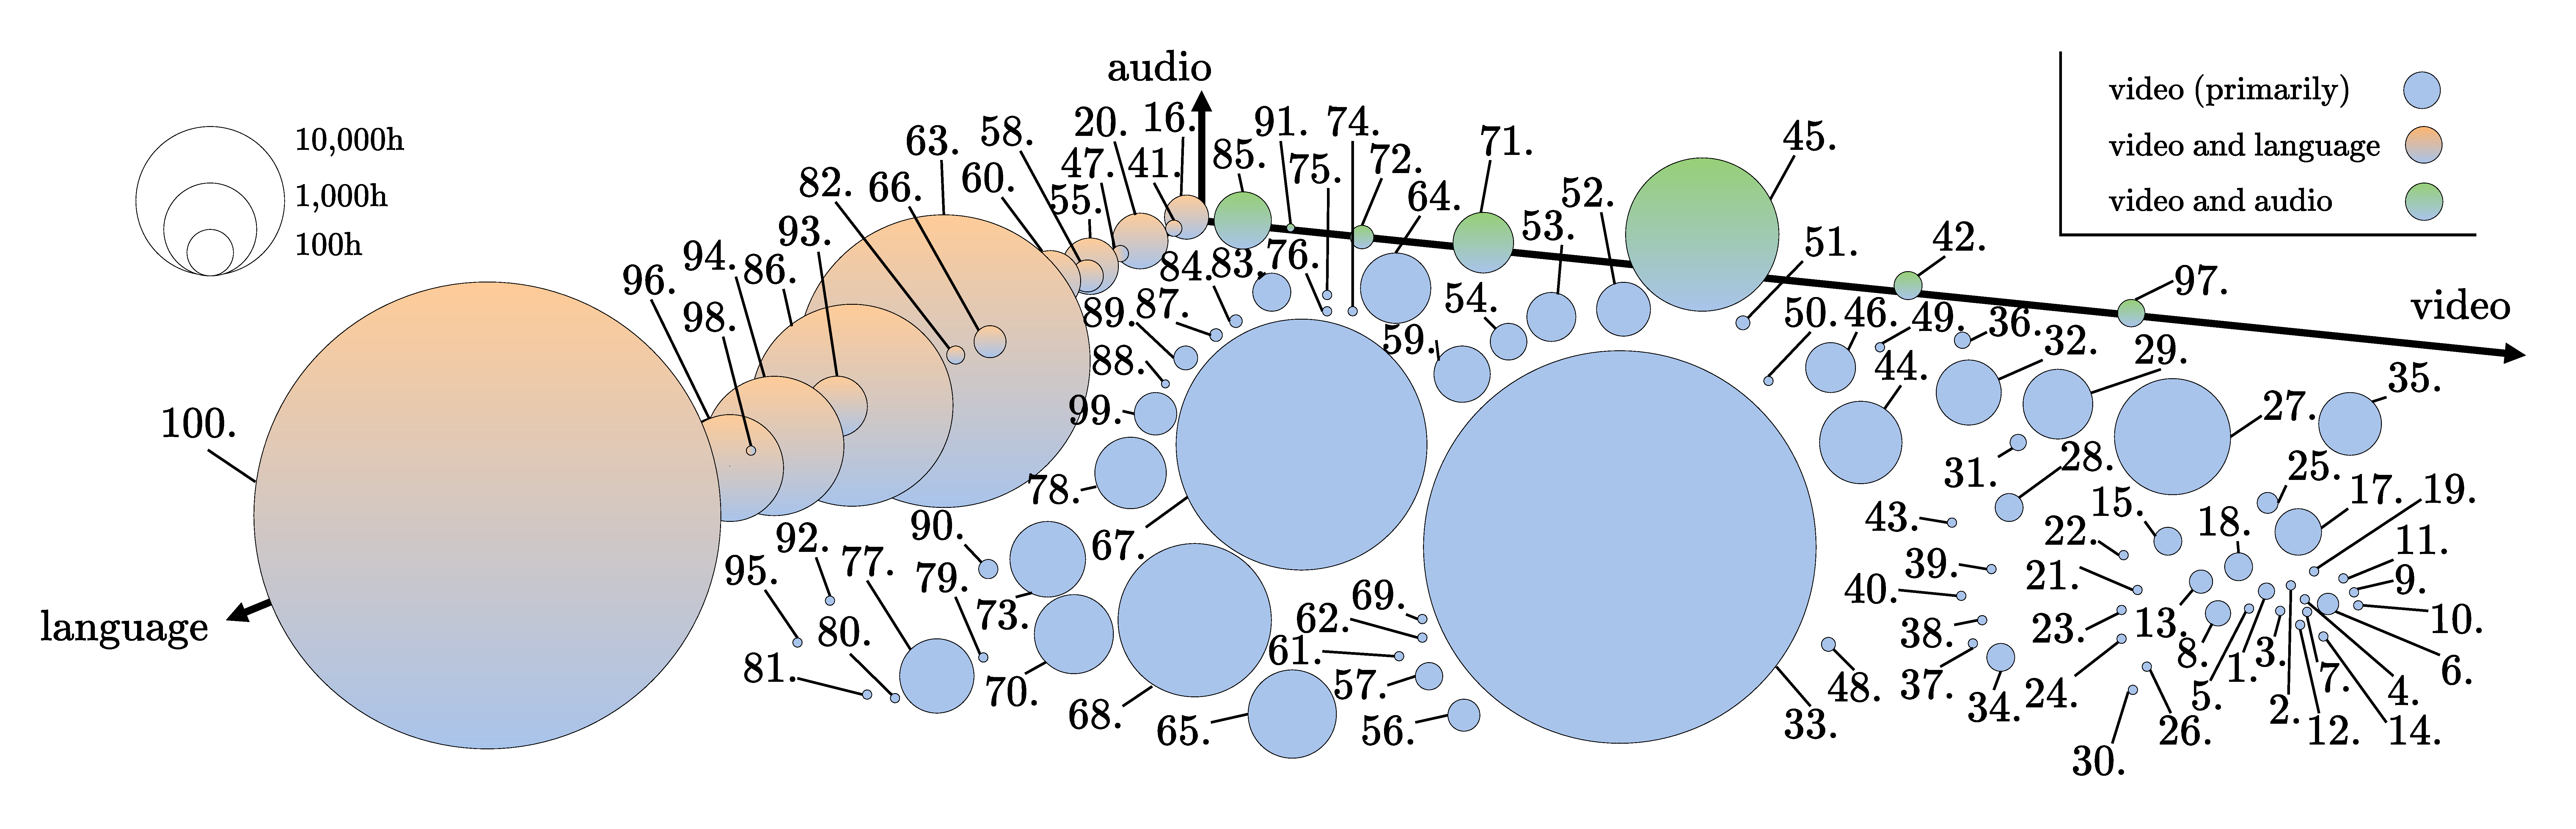
\includegraphics[width=\linewidth]{figs/datasets.pdf}
    \resizebox{\linewidth}{!}{
    \begin{tabular}{lllll}
      1. KTH~\citep{schuldt2004recognizing} &  
      2. Weizmann~\citep{gorelick2007actions} &  
      3. Coffee \& Cigarettes~\citep{laptev2007retrieving} & 
      4. CASIA Action~\citep{wang2007human} & 
      5. UCF Sports~\citep{rodriguez2008action} \\ 
      6. Hollywood~\citep{laptev2008learning} & 
      7. UT-Interaction~\citep{ryoo2009spatio} & 
      8. CMU-MMAC~\citep{deguide2008guide} &
      9. UCF-11~\citep{liu2009recognizing} & 
      10. Hollywood2~\citep{marszalek2009actions} \\ 
      11. TV-HI~\citep{patron2010high} &
      12. Humaneva~\citet{sigal2010humaneva} &
      13. UCF-50~\citep{reddy2013recognizing} & 
      14. Olympic Sports~\citep{niebles2010modeling} &
      15. HMDB-51~\citep{kuehne2011hmdb} \\
      16. MSVD~\citep{chen2011collecting} &
      17. CCV~\citep{jiang2011consumer} & 
      18. UCF-101~\citep{soomro2012ucf101} &
      19. CAD-60~\citep{sung2012unstructured} &
      20. MPII~\citep{rohrbach2012database} \\ 
      21. ADL~\citep{pirsiavash2012detecting} &
      22. 50 Salads~\citep{stein2013combining} &
      23. AVENUE~\citep{lu2013abnormal} &
      24. J-HMDB~\citep{jhuang2013towards} &
      25. CAD-120~\citep{koppula2013learning} \\
      26. Penn Action~\citep{zhang2013actemes} &
      27. Sports-1M~\citep{karpathy2014large} & 
      28. EGTEA Gaze+~\citep{li2015delving} &
      29. ActivityNet-100~\citep{caba2015activitynet} &
      30. Watch-n-Patch~\citep{wu2015watch} \\
      31. NTU-RGB-60~\citep{shahroudy2016ntu} &
      32. ActivityNet-200~\citep{caba2015activitynet} &
      33. YouTube-8M~\citep{abu2016youtube} & 
      34. Charades~\citep{sigurdsson2016hollywood} &
      35. ShakeFive2~\citep{van2016spatio} \\
      36. DALY~\citep{weinzaepfel2016towards} &
      37. OA~\citep{li2016recognition} &
      38. CONVERSE~\citep{edwards2016pose} &
      39. TV-servies~\citep{de2016online} & 
      40. Volleyball~\citep{ibrahim2016hierarchical} \\
      41. MSR-VTT~\citep{xu2016msr} &
      42. Greatest Hits~\citep{owens2016visually} &
      43. Okutama Action~\citep{barekatain2017okutama} &
      44. K-400~\citep{kay2017kinetics} &
      45. AudioSet~\citep{gemmeke2017audio} \\
      46. Smthng-Smthng (v1/v2)~\citep{goyal2017something} &
      47. TGIF~\citep{jang2017tgif} &
      48. CMU Panoptic~\citep{joo2017panoptic} &
      49. MultiTHUMOS~\citep{yeung2018every} &  
      50. RESOUND~\citep{li2018resound} \\
      51. EK-55~\citep{damen2018scaling} &
      52. K-600~\citep{carreira2018short} &
      53. VLOG~\citep{fouhey2018lifestyle} &
      54. AVA~\citep{gu2018ava} &
      55. TVQA~\citep{lei2018tvqa} \\
      56. UCF-Crime~\citep{sultani2018real} &
      57. Charades-Ego~\citep{sigurdsson2018charades} &
      58. YouCook2~\citep{zhou2018towards} &
      59. K-700~\citep{carreira2019short} &
      60. COIN~\citep{tang2019coin} \\
      61. AIST~\citep{tsuchida2019aist} &
      62. Drive\&act~\citep{martin2019drive} &
      63. HowTo100m~\citep{miech2019howto100m}&
      64. Moments in Time~\citep{monfort2019moments} &
      65. HACS~\citep{zhao2019hacs} \\
      66. VATEX~\citep{wang2019vatex} &
      67. IG65M~\citep{ghadiyaram2019large} &
      68. Toyota Smarthome~\citep{dai2022toyota} &
      69. OOPS~\citep{epstein2020oops} &
      70. AViD~\citep{piergiovanni2020avid} \\
      71. VGGSound~\citep{chen2020vggsound} &
      72. LLP~\citep{tian2020unified} &
      73. HVU~\citep{diba2020large} &
      74. DMP~\citet{ortega2020dmd} &
      75. Action Genome~\citep{ji2020action} \\
      76. Countix~\citep{dwibedi2020counting} &
      77. K-700 (2020)~\citep{smaira2020short} &
      78. FineGym~\citep{shao2020finegym} & 
      79. RareAct~\citep{miech2020rareact} &
      80. \citet{broxton2020immersive} \\
      81. HAA500 \citep{chung2021haa500} &
      82. IKEA ASM~\citep{ben2021ikea} &
      83. MultiSports~\citep{li2021multisports} &
      84. MOMA~\citep{luo2021moma} &
      85. Spoken Moments~\citep{monfort2021spoken} \\
      86. WebVid-2M~\citep{bain2021frozen} &
      87. Home action genome~\citep{rai2021home} & 
      88. DanceTrack~\citep{sun2022dancetrack} &
      89. EK-101~\citep{damen2022rescaling} &
      90. FineAction~\citep{liu2022fineaction} \\
      91. AVSBench~\citep{zhou2022audio} &
      92. \citet{li2022neural} &
      93. Assembly101~\citep{sener2022assembly101} &
      94. Ego4D \citep{grauman2022ego4d} &
      95. SportsMOT~\citep{cui2023sportsmot} \\
      96. Ego-Exo-4D \citep{grauman2024ego} & 
      97. EPIC-Sounds \citep{huh2023epic} &
      98. MVBench \citep{li2024mvbench} &
      99. OVR \citep{dwibedi2024ovr} &
      100. \citet{yang2024vidchapters}
    \end{tabular}
    }
    \caption{\textcolor{red}{TODO: datasets arranged in axes by their modality. Use cycle size to indicate total duration.}}
\end{figure*}

\subsection{General datasets}
\label{sec:datasets::general}
Over the past two decades, video datasets have scaled up the number of available videos and presented new and more robust baselines. We chronologically present widely-adopted benchmarks in~\Cref{tab:action_recognition_datasets}. Initial efforts \citep{schuldt2004recognizing,gorelick2007actions} have primarily focused on atomic actions such as categorizing \emph{walking}, \emph{running}, \emph{hand waving} etc. of low motion magnitudes. Later efforts before web-based crawling of videos in large-scale, the majority of datasets were comprised of videos from either TV shows and movies \citep{laptev2007retrieving,laptev2008learning,marszalek2009actions,patron2010high,kuehne2011hmdb} or sports \citep{rodriguez2008action,liu2009recognizing,reddy2013recognizing,niebles2010modeling}. A step towards establishing large-scale datasets for the video domain was made with the introduction of Kinetics \citep{carreira2017quo}, Sports-1M \citep{karpathy2014large}, and YouTube-8M \citep{abu2016youtube}, that included videos sourced from the web over diverse sets of actions. These datasets paved the way as general benchmarks for pertaining models that can be adapted for action-type-specific smaller datasets such as UCF-101 \citep{soomro2012ucf101} and ActivityNet \citep{caba2015activitynet}. In tandem, domains such as 
egocentric vision, human-object interactions, and hierarchical action understanding have also gained popularity prompting the creation of domain-specific datasets. EGTEA Gaze+ \citep{li2015delving}, EPIC KITCHENS \citep{damen2022rescaling}, and later EGO4D \citep{grauman2022ego4d} have been the main datasets and benchmarks for egocentric vision. Similarly, Something-Something \citep{goyal2017something} and Charades \citep{sigurdsson2016hollywood} have been used as benchmarks for object-based actions with a greater focus on temporal information. Datasets for semantic hierarchies include Diving-48 \citep{li2018resound} and FineGym \citep{shao2020finegym}. More recently datasets have also been created for subtasks that are adjacent to action recognition including; instruction learning \citep{alayrac2016unsupervised,bansal2022my,ben2021ikea,ohkawa2023assemblyhands,sener2022assembly101,tang2019coin}, action phase alignment \citep{sermanet2017unsupervised}, repeating action counting \citep{dwibedi2020counting,dwibedi2024ovr,hu2022transrac,runia2018real,zhang2020context}, action completion prediction \citep{epstein2020oops}, driver behavior \citep{martin2019drive,ortega2020dmd}, anomaly detection \citep{acsintoae2022ubnormal,liu2018future,lu2013abnormal,sultani2018real,wu2020not}, hand-object interactions \citep{chao2021dexycb,garcia2018first,hampali2020honnotate,kwon2021h2o,moon2020interhand2,mueller2017real}, and object state changes in actions \citep{souvcek2022look}.



\subsection{Task- and modality-specific datasets}
\label{sec:datasets::specific}

Apart from general-purpose datasets, benchmarks have also been proposed for specific aspects of action understanding. We overview three groups of tasks and benchmarks based on the holistic understanding of scenes beyond standard monocular videos and the use of supplementary modalities to video such as language and audio. 

% Multi-view and multi-camera set-ups
\noindent
\textbf{Multiview}. The human visual system can perceive the world around us in great detail. Usually, this detail comes from head movements that change the viewer's perspective and improve a scene's holistic understanding. 
Initial efforts compiled multi-view videos from a small number of subjects \citep{sigal2010humaneva} or through synthetic data \citep{ionescu2013human3}. Capturing high-quality multi-view videos is highly dependent of the hardware and setup. CMU panoptic \citep{joo2017panoptic} captures group interactions with a geodesic dome with 480 VGA cameras. Interactions included social settings, games, dancing, and musical performances. Similarly, ZJU-Mocap \citep{peng2021neural} comprises dynamic videos of human motions from 20 cameras. More recently, the Immersive Light Field dataset \citep{broxton2020immersive} collected light field videos with 6 degrees of freedom with a camera rig consisting of 46 action cameras. Multi-view datasets have also been collected for varying target tasks 3D video synthesis of human actions and interactions in indoor \citep{li2022neural} and outdoor \citep{lin2021deep,yoon2020novel} settings, dance sequence reconstruction \citep{tsuchida2019aist}, and the dyncamic synthesis of indoor spaces that actions take place \citep{tschernezki2024epic}.

% Language-related tasks
\noindent
\textbf{Video-language}. In recent years language has been integrated into vision tasks as a natural extension to represent high-level semantics. Commonly, learning to map textual concepts and visual representations in a shared embedding space has been a widely adopted strategy by many video tasks \textcolor{red}{TODO refs}. Initial video-language datasets \citep{chen2011collecting,xu2016msr} were based on short video snippets and short textual descriptions of actions performed over the video. Recent efforts have also provided multilingual descriptions \citep{wang2019vatex}. Video question-answering is another popular language-based task that has been explored by a large number of works. \citep{jang2017tgif,lei2018tvqa,li2024mvbench,oncescu2021queryd,xiao2021next}. For long videos, The sequentiality of instructions has been of great interest with the introduction of benchmarks such as HowTo100M \citep{miech2019howto100m}, YouCook2 \citep{zhou2018towards}. Benchmarks have also been proposed for other long-form tasks such as moment retrieval \citep{song2024moviechat,yang2024vidchapters}, and long-term reasoning \citep{mangalam2023egoschema}.

% Video and audio
\noindent
\textbf{Audio and vision}. Human perception has often relied on both vision and audio for perceiving actions, especially in conditions where appearance may lead to ambiguous predictions. Audioset \citep{gemmeke2017audio} is the largest audio-visual dataset containing 2.1M clips across a long-tail distribution of 527 classes. VGG-Sound \citep{chen2020vggsound} is another common benchmark with 200K videos uniformly distributed across 300 classes. Datasets have also been collected for specific tasks such as audio-visual semantic segmentation \citep{zhou2022audio}, audio-visual video parsing \citep{tian2020unified}, materials sound and action classification \citep{huh2023epic,owens2016visually}, and video captioning \citep{monfort2021spoken}.




\section{From recognition to research tasks}
\label{sec:recognition}

\citep{wang2023learning}s

\subsection{Temporal-based tasks}

\citep{albanie2020end}
\citep{stergiou2023leaping}


\begin{figure}[t]
     \centering
     \begin{subfigure}[b]{0.49\linewidth}
         \centering
         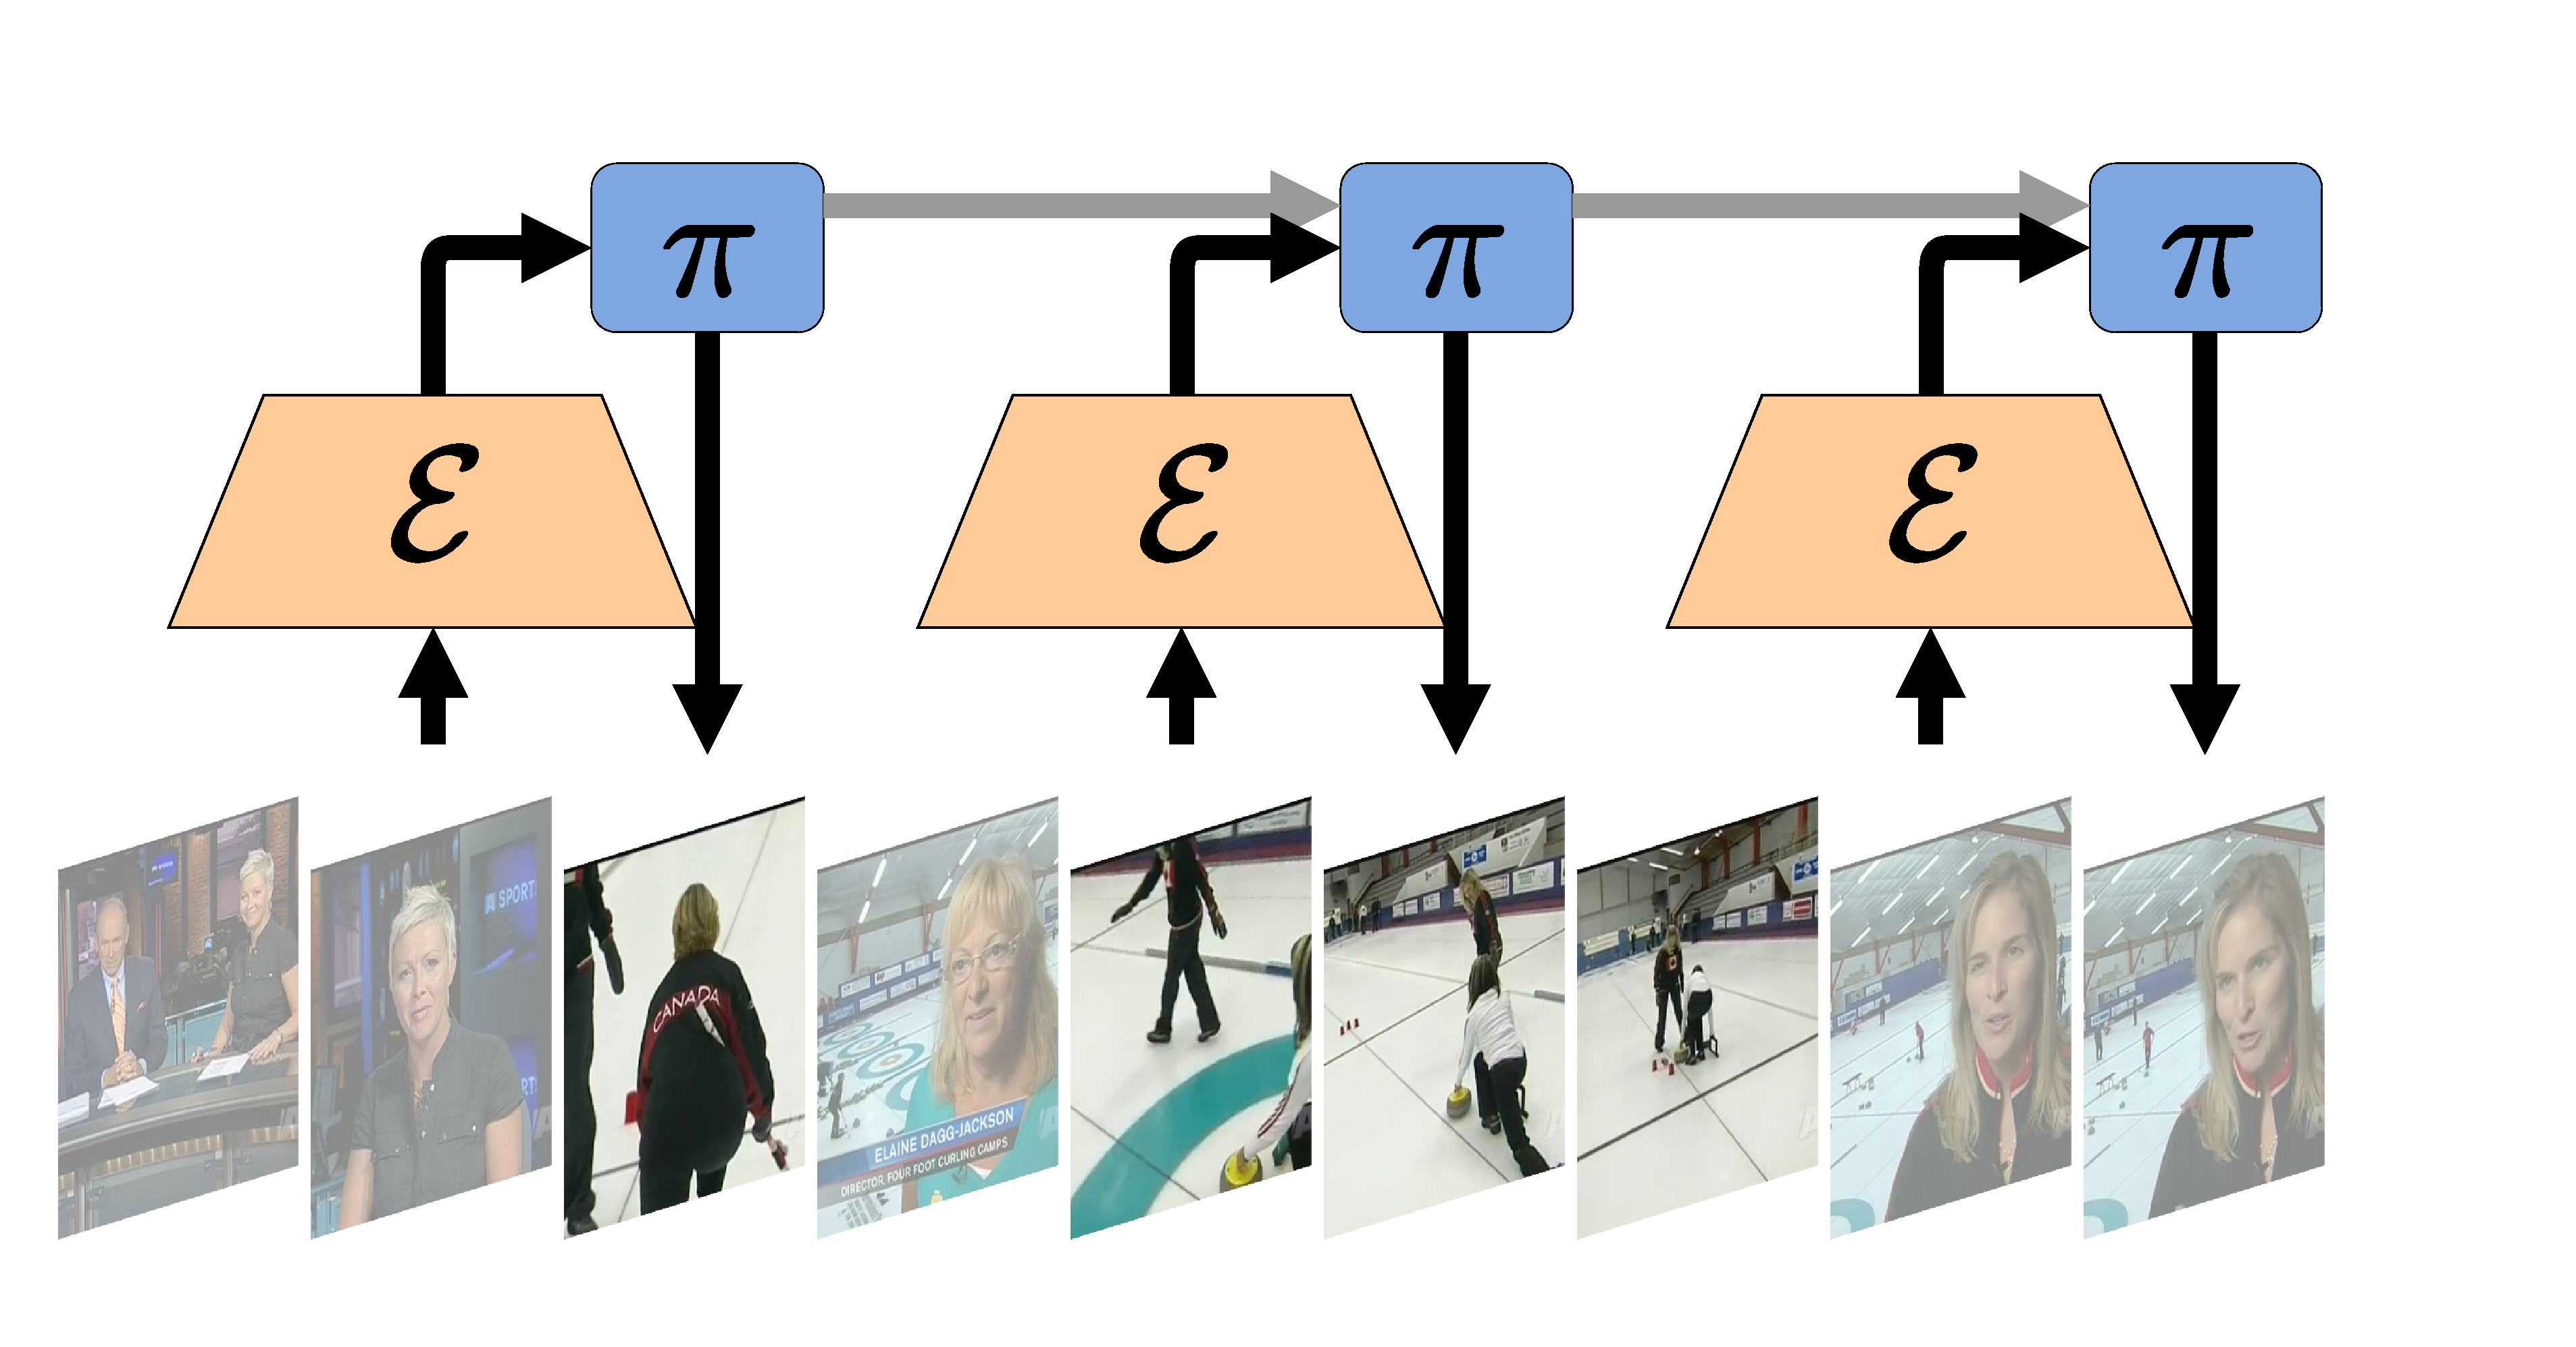
\includegraphics[width=\linewidth]{figs/redundancies_reduction/redudancies_sample.pdf}
         \caption{\textbf{Frame Sampling}}
         \label{fig:redundancies_reduction::sampling}
     \end{subfigure}
     \hfill
     \begin{subfigure}[b]{0.49\linewidth}
         \centering
         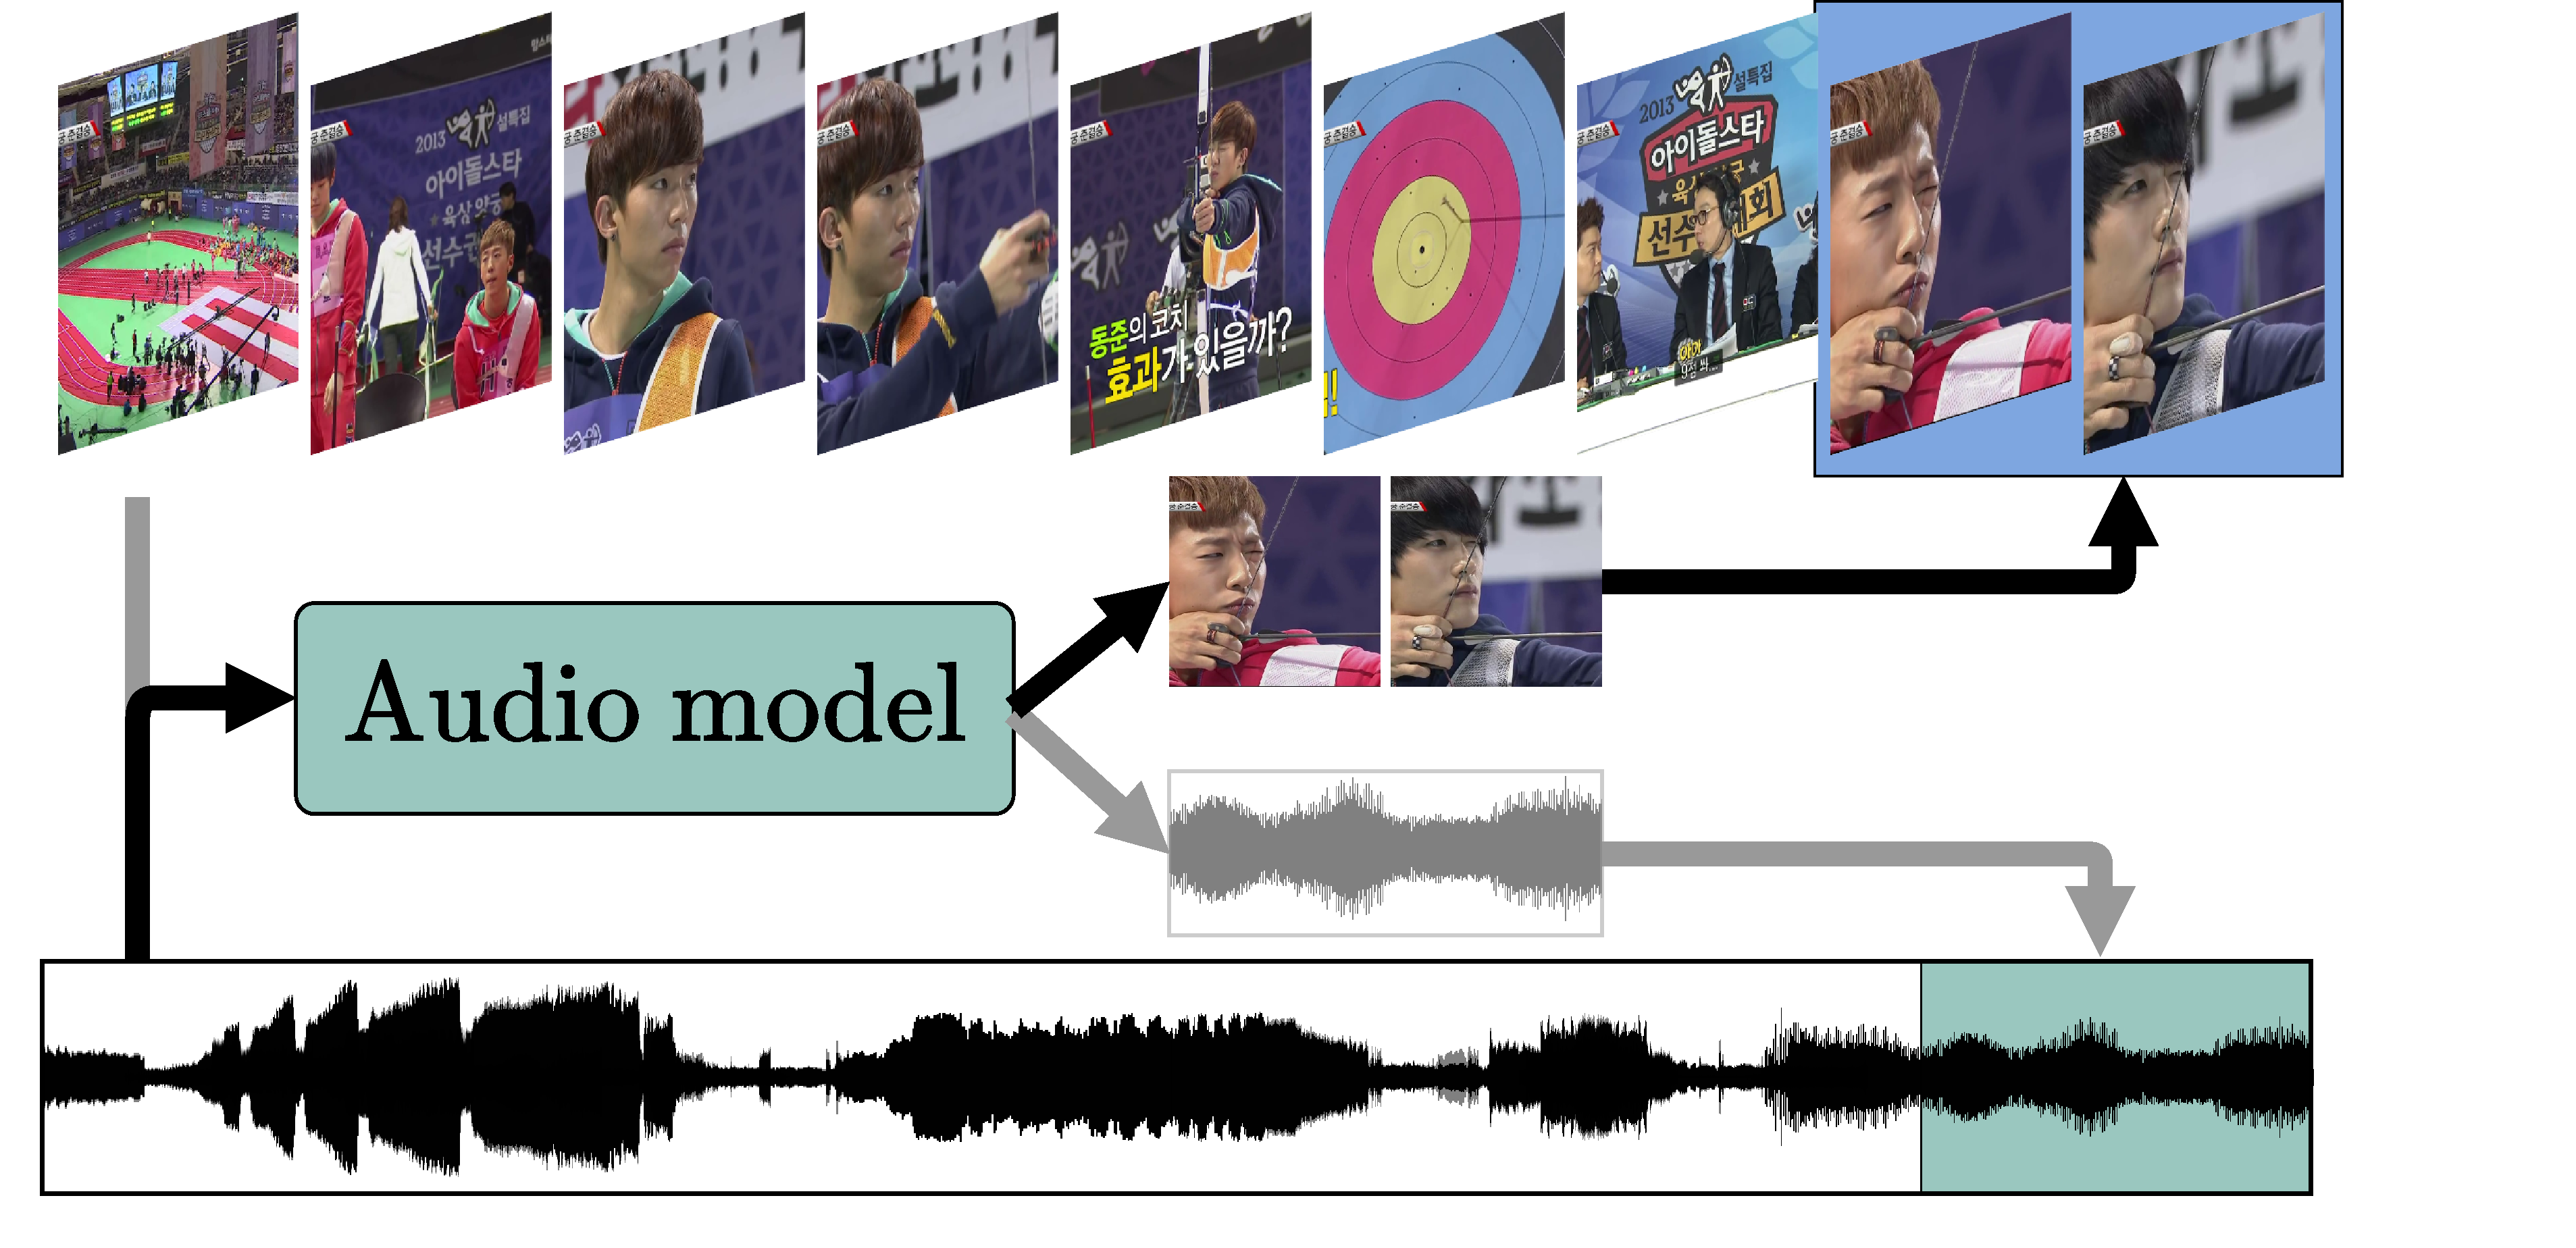
\includegraphics[width=\linewidth]{figs/redundancies_reduction/redudancies_preview.pdf}
         \caption{\textbf{Audio previewing}}
         \label{fig:redundancies_reduction::preview}
     \end{subfigure}
     \\
     \begin{subfigure}[b]{0.49\linewidth}
         \centering
         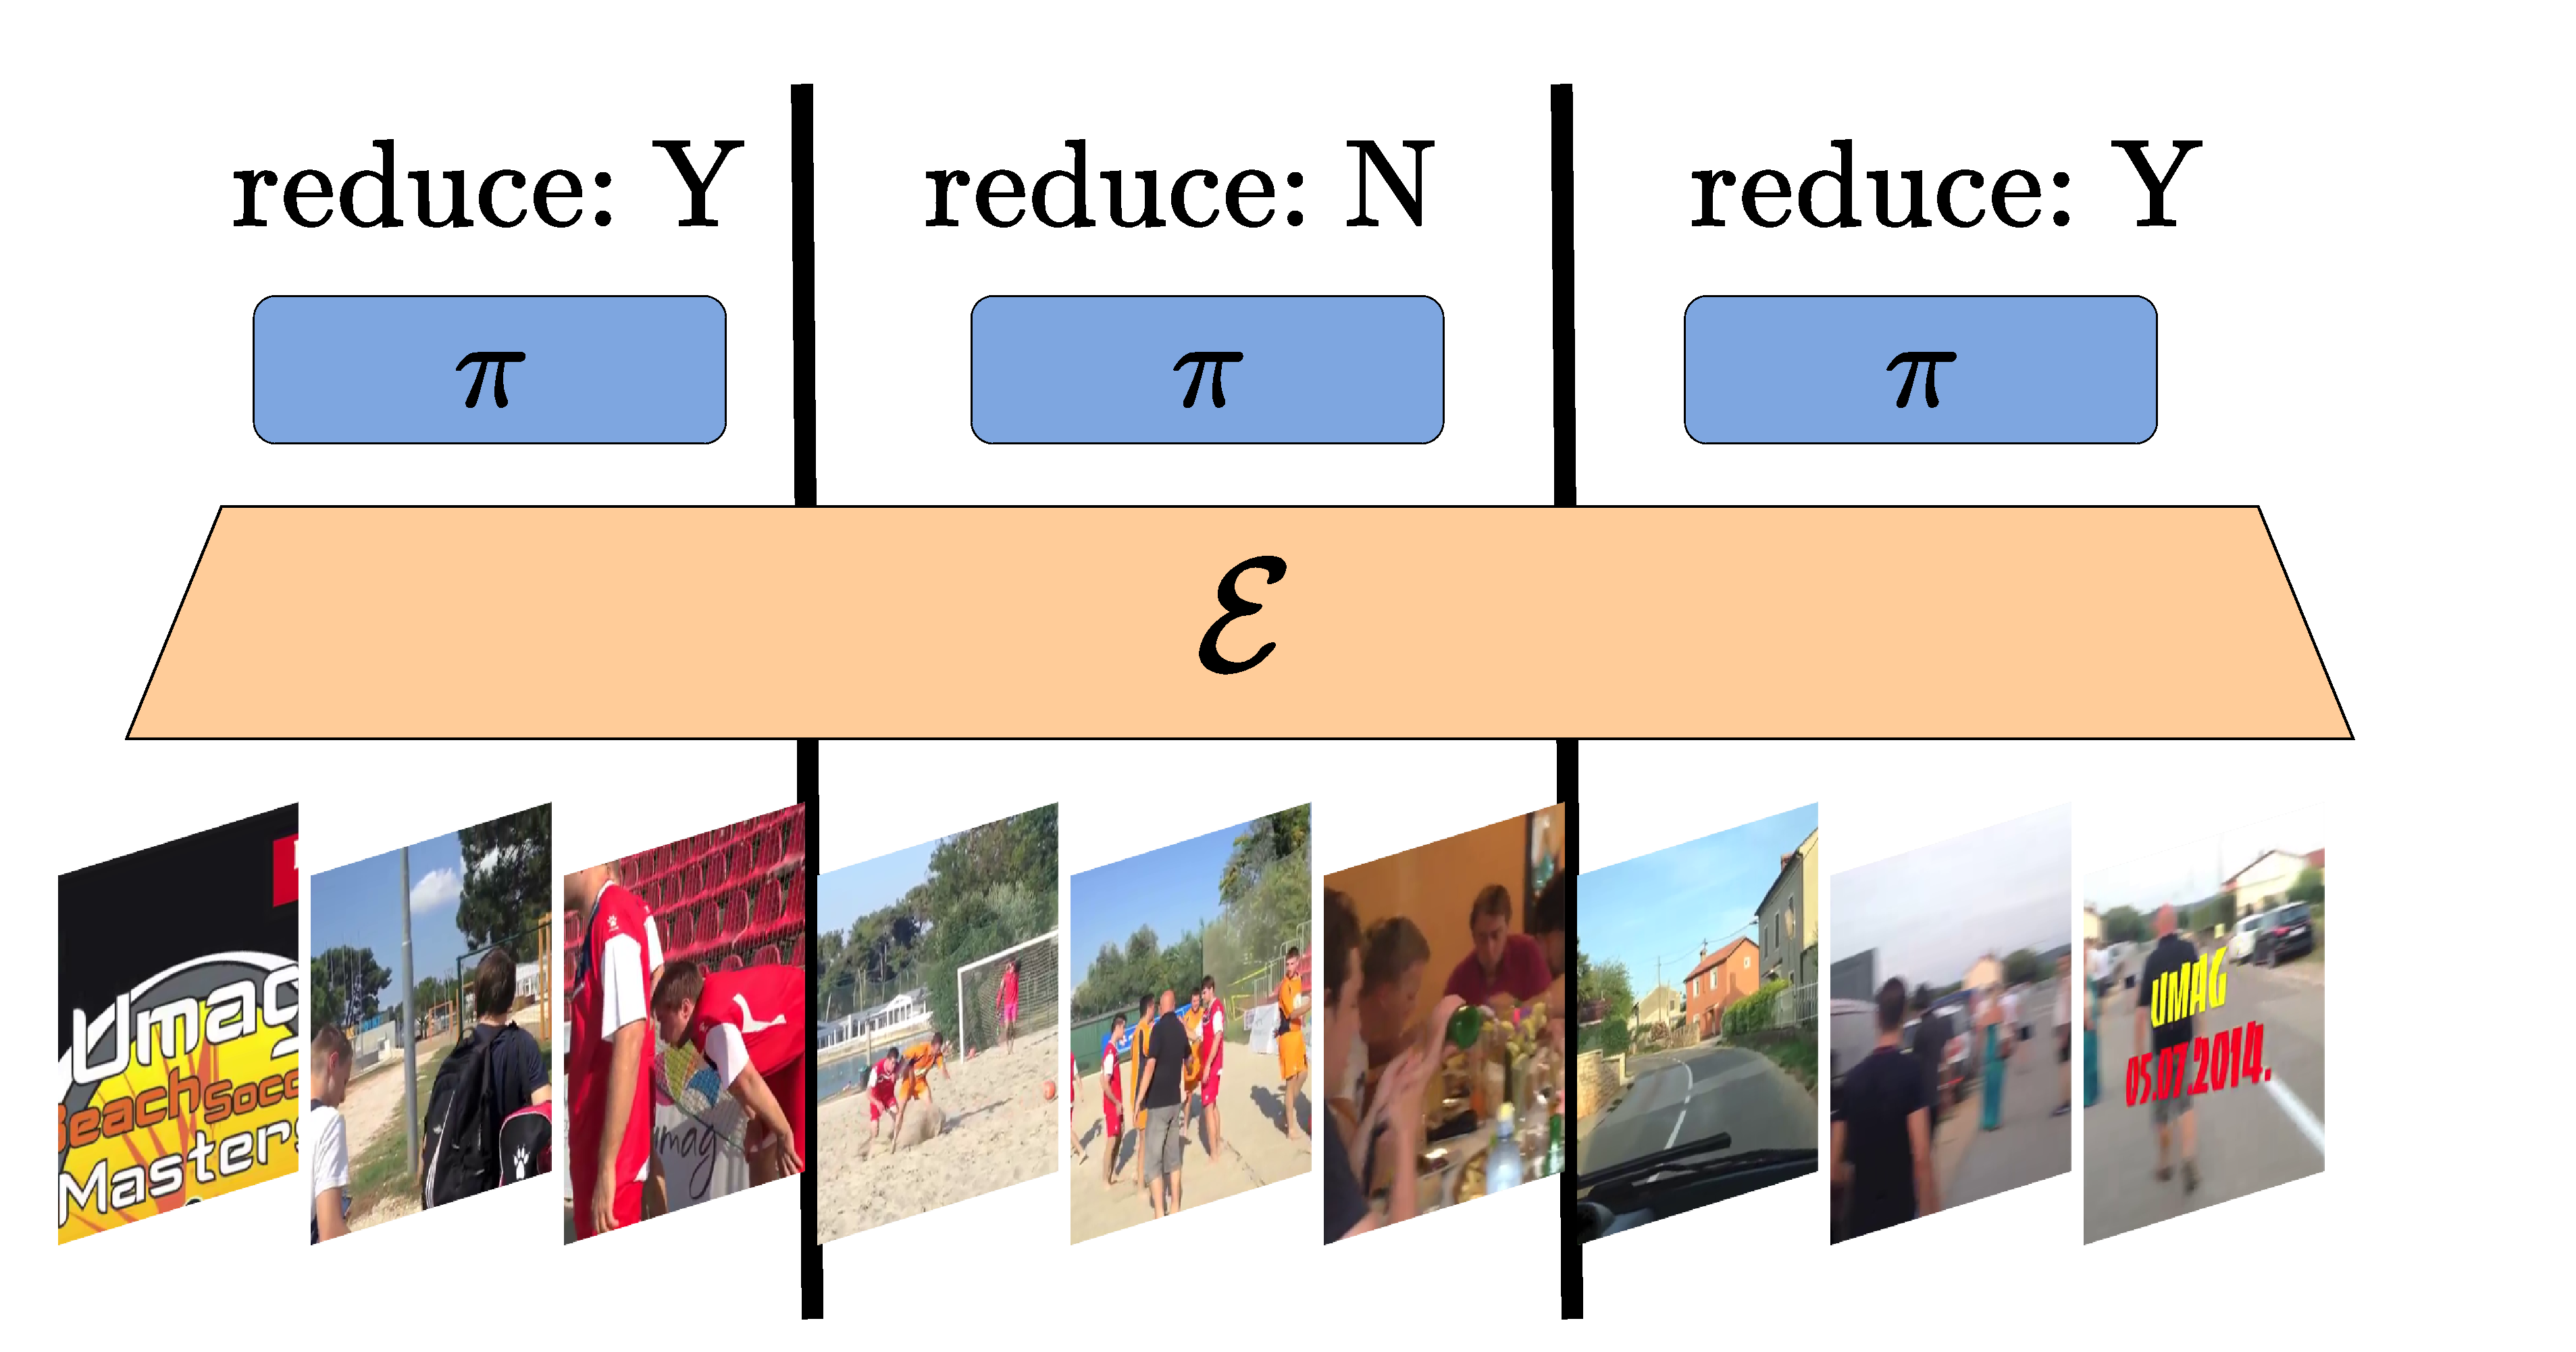
\includegraphics[width=\linewidth]{figs/redundancies_reduction/redudancies_permute.pdf}
         \caption{\textbf{Video input permuting}}
         \label{fig:redundancies_reduction::permute}
     \end{subfigure}
     \hfill
     \begin{subfigure}[b]{0.49\linewidth}
         \centering
         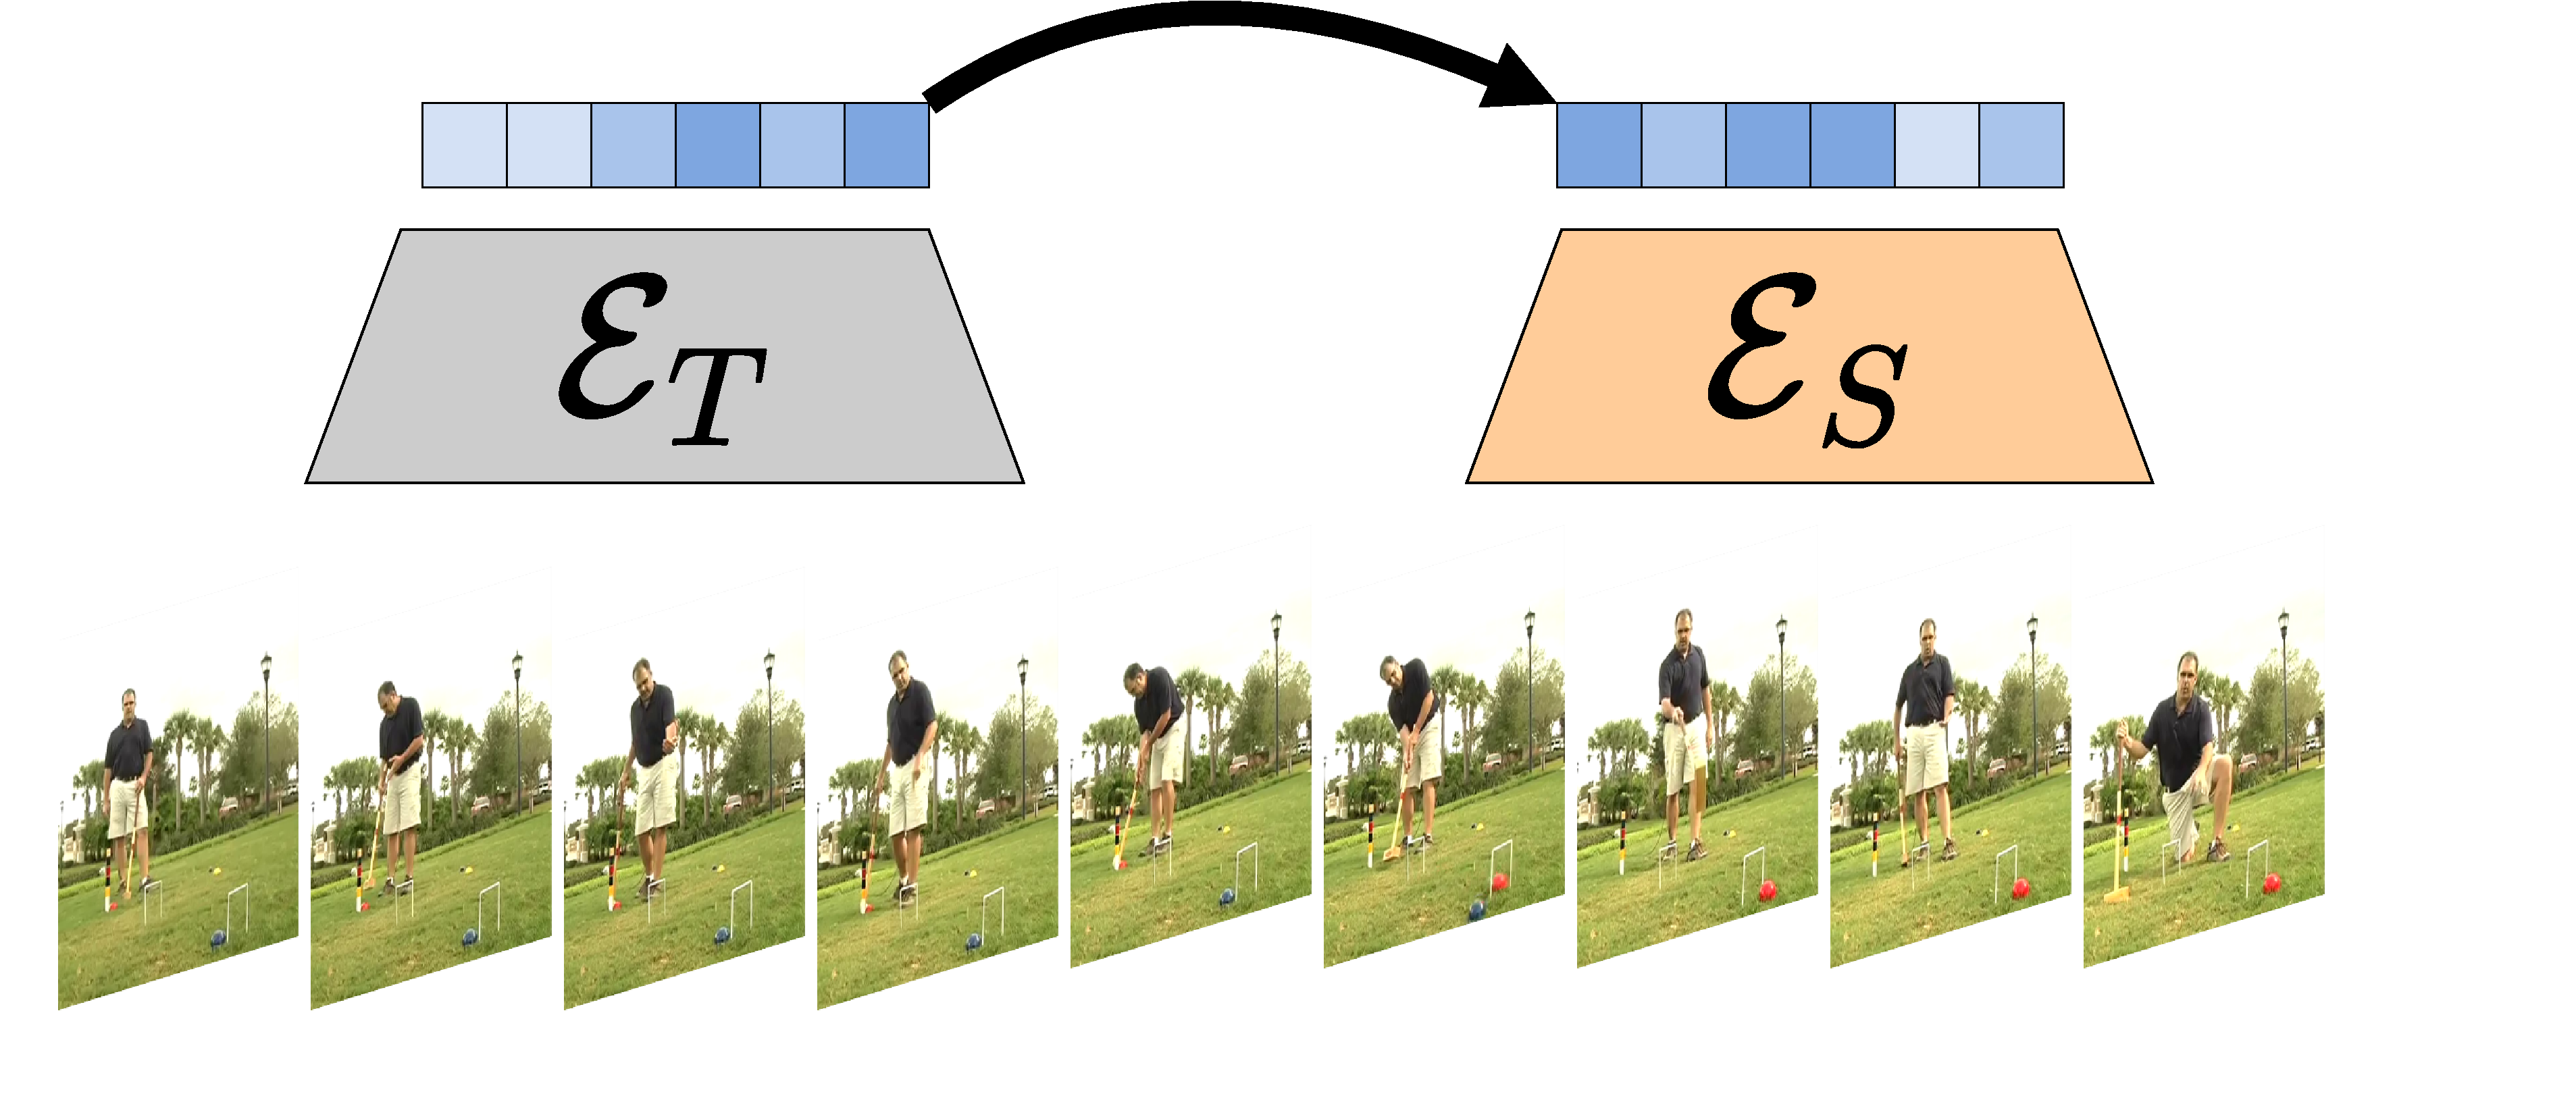
\includegraphics[width=\linewidth]{figs/redundancies_reduction/redudancies_transfer.pdf}
         \caption{\textbf{Knowledge transfer}}
         \label{fig:redundancies_reduction::transfer}
     \end{subfigure}
        \caption{\textbf{Redudency reduction methods overview} \textcolor{red}{To update}}
        \label{fig:redundancies_reduction}
\end{figure}

% Main challenges in AR
\noindent
\textbf{Challenges}.


% Why sample/reduce compute?
\noindent
\textbf{Reducing redundancies in recognition}. Based on a 2024 study \citep{sandvine2024global}, video accounts for over 5 exabytes of the world's daily internet traffic. 

% Frame sampling
As the efficient processing of videos can be a computational burden, works have focused on reducing redundancies. One of the most common approaches for reducing redundancies is \emph{frame sampling}. Works on frame sampling rely on policy networks over videos selecting frames based on the action's complexity \citep{ghodrati2021frameexit,yeung2016end}, correspondence with the video's context \citep{wu2019adaframe}, or changes in the target class' probability \citep{korbar2019scsampler}. \citet{wang2021adaptive} used a recurrent network to localize action-relevant regions with further extensions including early stopping \citep{wang2022adafocus} and features from the entire video to determine the action-relevant patch coordinates \citep{wang2022adafocusv3}. \citet{xia2022nsnet} classified frames as salient and non-salient by pseudo labels obtained by embedding distance to class centroids. Other approaches have used reward functions based on predictions from the selected frames \citep{wu2020dynamic}, combined frame-level and video-level predictions \citep{gowda2021smart}, optimized towards balancing accuracy and number of frames used \citep{wu2019liteeval}, or removed tokens in transformer architectures \citep{wu2024haltingvt}.

% Sampling by using an additional low-cost signal
A more recent adjacent set of approaches has been based on frame sampling by \emph{previewing audio}. \citet{gao2020listen} used both frame and audio features with a recurrent network to predict the next informative moment in the video. Similarly, \citet{nugroho2023audio} used soft predictions to localize salient audio segments from which the corresponding parts of the video can be selected. 

% Permuting the input (w/o sampling) to improve efficiency
Although sampling can be a beneficial technique in short videos, as the context of videos increases, using a small number of frames can result in information loss. Another line of research thus studies redundancies reduction by \emph{video input permutations}. These works either change frame resolutions based on classifier confidence \citep{meng2020ar} or quantize frames at different precision \citep{abati2023resq,sun2021dynamic}. \citet{zhang2022look} used a two-branch approach for light computations larger context and heavier computations in a smaller context similar to \citep{feichtenhofer2019slowfast}.  

% Using teacher model embeddings
Recent efforts have also used \emph{knowledge distillation} to improve the training efficiency of video model pipelines. Works have focused on learning to match reduced resolution features from the student to full resolution teacher features \citep{ma2022rethinking}, or cross-attended between teacher and student features during training \citep{kim2021efficient}. Distillation approaches have also used teacher models from additional modalities. \citet{lei2021less} bound language embeddings to sparsely sampled clips from long videos. \citet{xia2022temporal} used embeddings from textual event-object relations to discover salient frames. \citet{tan2023egodistill} proposed a reconstruction approach for interpolating egocentric video features using embeddings from partial frames and the camera motion for the unobserved frames.


\begin{figure*}[t]
    \centering
    \begin{overpic}[width=\linewidth, trim={0 17cm 0 5cm},clip]{figs/localization_detection_counting.pdf}
    \put (15,0) {(a) TAL}
    \put (43,0) {(b) STAD}
    \put (71,0) {(c) VRC}
    
    \end{overpic}
    \caption{\textbf{Objective visualization for Temporal Action Localization (TAL), Spatio-Temporal Action Detection (STAD), Video Repetition Counting (VRC)}. TAL (a) discovers the start and end times of individual actions. In contrast, STAD (b) is more complex as it requires temporally and spatially localizing actions with bounding boxes for actors and objects over time. Distinctively, VRC (c) is not based on action labels and instead requires counting repetitions of actions or motions in an open-set setting. Video source from \citep{kay2017kinetics}.}
    \label{fig:loc_det_count}
\end{figure*}

% TAL definition and early works
\noindent
\textbf{Temporal localization}. A well-established video task is discovering and classifying temporal segments and the actions performed. Temporal Action Localization (TAL) aims to infer the classification label alongside the start and ends of the corresponding locations in untrimmed videos. Early attempts have used Improved Dense Trajectories \citep{wang2013action} and Fisher Vector \citep{oneata2013action} to model the temporal dynamics of scenes. \citet{shou2016temporal} was one of the first to approach TAL by defining a joint action proposal and classification objective to optimize a regional CNN. This joint optimization has been adapted in subsequent works to use spatial and temporal-only networks \citep{lin2018bsn,paul2018w,wang2017untrimmednets}, regional proposal selection \citep{chao2018rethinking,xu2017r}, or intra-proposal relationships with graph convolutions \citep{zeng2019graph}. \citet{shou2017cdc} predicted granularities at a frame level by transposing the temporal resolution of pre-trained video encoders. More recent approaches for TAL can be categorized into three broad categories. 

% Single-stage approaches
Most similar to the aforementioned methods, \textbf{one-stage} approaches, localize and classify actions in a single step using hierarchical embeddings from feature pyramids \citep{lin2021learning,liu2020progressive,shi2023tridet,zhang2022actionformer} or discovering segments by relating relevant videos \citep{shou2018autoloc,yang2020localizing}. Recently, \citet{yan2023unloc} has also introduced the use of vision-language encoders for encoding and using the scene's semantic context for TAL. As the definition of specific start and end frames for actions can often be ambiguous, a set of approaches have relaxed their objectives to weigh the training loss by the importance of each frame within the action segment \citep{shao2023action} or
learning distributions of possible start and end times \citep{moltisanti2019action}. 

% Two-stage approaches
In a different line of research, a group of methods use additional steps to regress temporal boundaries. One line of \textbf{two-stage} approaches disentangles the optimization into separate parts. \citet{zhai2020two} combined proposals from spatial- and temporal-only streams into a fused final prediction. \citet{chen2022dcan} used long- and short-range temporal information to refine the confidence of the generated action proposals. \citet{huang2019decoupling} decoupled classification and localization to two objectives during training with two separate models that use cross-modal connections for exchanging information. Approaches have also aimed to maximize the embedding difference between representations of frames from action segments and non-relevant frames either with positive and negative instances \citep{luo2020weakly,zhang2021cola} or by a scoring function \citep{rizve2023pivotal}. Methods have also improved the features of backbone encoders with more TAL-relevant pretext tasks \citep{zhang2022unsupervised}. Most two-step methods however process videos holistically \citep{alwassel2021tsp,he2022asm,liu2021weakly,qing2021temporal}. \citet{alwassel2021tsp} encode local features over a sliding window. Use aggregated features from all local encoders to find the regions of action while classifying every segment. Graphs have also been adopted for TAL with \citet{bai2020boundary} using generated candidate proposals for the graph's start/end edges and its connected nodes. \citet{zhao2021video} created a graph of hierarchical features with windows over multiple temporal resolutions. More recent approaches \citep{nag2023difftad} have also formulated proposal prediction as a denoising task with noisy action proposals as input to a diffusion model conditioned on the video.

% Encoder-decoder/DETR
A recent set of methods has been based on adapting \textbf{DEtection TRansformers DETR} \citep{carion2020end} to TAL. DETR-based approaches rely on transformer encoder-decoders to create regional proposals that can be in turn optimized with bipartite matching. \citet{tan2021relaxed} adapted DETR with a matching scheme of multiple positive action proposals to address sparsity in temporal annotations. Works that aimed towards optimization have included dense residual connections \citep{zhao2023re2tal} or caching short-term features \citep{cheng2022tallformer,hong2022spotting}. 
\citet{liu2024end} have scaled model capacity upwards by training intermediate adaptors to propagate information to the decoder from intermediate frozen encoder layers. Approaches have also explored training recipes with sparsely updating model layers \citep{cheng2022stochastic}, vision-language pre-training distillation \citep{ju2023distilling}, proposal hierarchies \citep{wu2023newsnet},
and end-to-end TAL encoder-decoder optimization \citep{liu2022empirical}. 




\noindent
\textbf{Spatiotemporal detection}. Adding to TAL, SpatioTemporal Action Detection (STAD) is more complex as it localizes the temporal extend of actions and detects action-relevant actors and objects over frames. Maintaining consistency between the per-frame detections and the temporal action proposals in the main challenge of STAD methods. Similar to the research directions for localization, two categories can be used to overview relevant literature. 


Bulding upon the advancements of image-based object detectors \citep{girshick2014rich,girshick2015fast}, the majority of approaches perform STAD in \textbf{two stages} by first detecting objects and then temporally localizing action by tracking object candidates~\citep{jain2014action,weinzaepfel2015learning}, ROI-pooling rgb and flow features \citep{peng2016multi}, refining proposals iteratively \citep{soomro2015action}, aligning source and target domain features~\citep{agarwal2020unsupervised}, or using the general action level in the video as context \citep{mettes2016spot}. \citet{li2018recurrent} build upon prior two-stage detection with the incorporation of recurrent proposals to include temporal context. Other refining approaches \citep{singh2017online} used the arrow of time with different portions of the video detected at each step. The introduction of benchmarks with videos of higher temporal resolutions \citep{gu2018ava} also led approaches towards including additional context over longer frame sequences with future banks \citep{feng2021relation,pan2021actor,tang2020asynchronous,wang2018videos,wu2019long,wu2022memvit} or additional objects \citep{arnab2021unified,hou2017tube,zhang2019structured} which has showed further improvements in detection capabilities of models. Additional information such as keyframe saliency maps~\citep{li2020actions,ulutan2020actor}, hands and poses~\citep{faure2023holistic}, actor-object relations~\citep{sun2018actor}, self-supervision~\citep{wang2023videomae} have also been explored. \citet{alwassel2018diagnosing} analyzed the advancements of two-stage approaches beyond performance metrics showing that improvements are centered towards handling temporal context. However, features used are pre-computed from large backbones requiring auxiliary task-specific models.  


Drawing inspiration from \textbf{single-stage} object detection methods~\citep{carion2020end,redmon2016you,liu2016ssd}, STAD single-stage approaches use a unified framework for both localization and detection~\citep{chen2021watch,girdhar2019video,zhu2024dual}. \citet{ntinou2024multiscale} extended the bipartite matching loss from \citet{carion2020end} to spatio-temporal tokens. Other approaches also used adaptive feature sampling~\citep{wu2023stmixer}, conditioning modeled visual features based on motion~\citep{zhao2019dance}, or have contrasted different views in training~\citep{kumar2022end}. Directly predicting tubelets has also been adopted as as a recent direction by recent approaches~\citep{gritsenko2024end,kalogeiton2017action,song2019tacnet,yang2019step,zhao2022tuber}. \citet{kalogeiton2017action} stacked embeddings from a backbone used in a sliding window to regress classes and tubelets over the entire video. \citet{zhao2022tuber} used an encoder-decoder to generate tubelet queries and cross-attended them to visual features. \citet{gritsenko2024end} generated a candidate tubelet based on a condensed query representation used to cross-attend with features at each frames. Beyon STAD, tubelets have also been used are a self-similarity pre-training objective~\citep{thoker2023tubelet} to enforce correspondence of videos from different domains but with similar local motions. 





\noindent
\textbf{Repetition counting}. Relating to TAL and STAD, Video Repetition Counting (VRC) approaches aim to count the number of action repetitions. In contrast to TAL/STAD however, VRC is an open-set task and does not require temporally localizing actions. Early works relied on the periodicity of signals \citep{thangali2005periodic} decomposing the repetitions of signals with a Fourier analysis \citep{branzan2008generic,briassouli2007extraction,ousman2008segmentation,ross2000robust,pogalin2008visual}. Signal-based works have used the flow directions over time \citep{runia2018real}. A number of approaches have defined VRC as a classification task. \citet{lu2004repetitive} used dynamic parameters based on the Frobenius norm to classify changes corresponding to action end times.
\citet{zhang2021repetitive} fused audio and video representations while \citet{zhang2020context} used multiple cycles to refine the repetition count prediction. \citet{li2024efficient} extracted action query features and classified the queries for repeating actions. In contrast to defining a classification task with a predefined number of possible repetitions, \citet{dwibedi2020counting} adopted a temporal self-similarity matrix \citep{benabdelkader2004gait,junejo2010view,korner2013temporal} to discover the periodicity of repetitions. Subsequent methods have used embedding similarity matrices with multiple scales \citep{bacharidis2023repetition,hu2022transrac}, triplet contrastive losses \citep{destro2024cyclecl}, and graph representations \citep{panagiotakis2018unsupervised}. As representations can be highly similar for adjacent frames, several recent methods have instead aimed to limit the discovery of correspondences in repetition instances to poses \citep{ferreira2021deep,yao2023poserac}, specific frames \citep{li2024repetitive,zhao2024skim}, visual exemplars \citep{sinha2024every}, or language descriptions \citep{dwibedi2024ovr}.

\noindent
\textbf{Future outlooks}.

\noindent
\subsection{Multitask optimization}

cross-dataset
\citep{perrett2019ddlstm}
\citep{kapidis2019multitask} 
\citep{bansal2024videocon}



\begin{figure*}[t]
    \centering
    \includegraphics[width=\linewidth,height=5cm]{example-image-a}
    \caption{\textcolor{red}{TODO: Table for grouped language approaches.}}
\end{figure*}


\subsection{Language semantics in videos}
\citep{song2024moviechat}
\citep{yu2017end}
\citep{anderson2018vision}

\citep{xu2021videoclip}
\citep{ashutosh2023hiervl}
\citep{kahatapitiya2024victr}
\citep{li2023videochat}
\citep{jiang2023motiongpt}
\citep{bain2021frozen}
\citep{fu2021violet}
\citep{han2022temporal}
\citep{ko2022video}
\citep{lei2021less}
\citep{li2022align}
\citep{li2020hero}
\citep{miech2020end}
\citep{seo2022end}
\citep{seo2021look}
\citep{sun2019videobert}
\citep{wang2023all}
\citep{wang2022object}
\citep{zellers2021merlot}
\citep{lei2021detecting}
\citep{lin2022egocentric}
\citep{wang2022contrastive}
\citep{zhu2020actbert}

\citep{zhao2024videoprism}
\citep{cheng2024egothink}
\citep{wang2024omnivid}
\citep{kuo2023mammut}

\noindent
\textbf{Video Question Answering (VideoQA)}
\citep{xue2023egocentric} 
\citep{min2024morevqa}
\citep{yang2022zero}
\citep{yang2021just}
\citep{yang2022learning}
\citep{xiao2021next}
\citep{xu2017video}
\citep{zhang2023video}
\citep{yu2023self}
\citep{xiao2024can}
\citep{gao2023mist}
\citep{xiao2022video}
\citep{xiao2023contrastive}
\citep{li2022equivariant}
\citep{li2023discovering}
\citep{jiang2020reasoning}
\citep{park2021bridge}
\citep{guo2021multi}
\citep{jang2017tgif}
\citep{fan2019heterogeneous}
\citep{gao2018motion}
\citep{huang2020location}
\citep{li2019beyond}
\citep{liu2021hair}
\citep{dang2021hierarchical}
\citep{cherian20222}
\citep{geng2021dynamic}
\citep{ye2017video}
\citep{zeng2017leveraging}



\noindent
\textbf{Video Captioning} \ding{52} 
\citep{alayrac2022flamingo}
\citep{krishna2017dense}
\citep{yang2023vid2seq}
\citep{chen2024panda} 
\citep{ren2024timechat} 
\citep{zhou2024streaming}
\citep{islam2024video}
\citep{mavroudi2023learning}
\citep{iashin2020better}
\citep{iashin2020multi}
\citep{wang2018bidirectional}
\citep{wang2020event}
\citep{chen2021towards}
\citep{deng2021sketch}
\citep{mun2019streamlined}
\citep{rahman2019watch}
\citep{shen2017weakly}
\citep{shi2019dense}
\citep{wang2021end}
\citep{zhou2018end}
\citep{han2023autoad}
\citep{han2023autoadii}
\citep{han2024autoadiii}
\citep{seo2022end}
captioning multitask
\citep{chadha2021iperceive}
\citep{li2018jointly}


\noindent
\textbf{Video Retrieval} \ding{52}
\citep{gordo2017beyond}
\citep{wang2016learning}
\citep{xu2015jointly}
\citep{torabi2016learning}
\citep{dong2018predicting}
\citep{otani2016learning}
\citep{kim2024you} 
\citep{wray2019fine} 
\citep{wray2021semantic}
\citep{ge2022bridging}
\citep{xue2022advancing}
\citep{gabeur2020multi}
\citep{mithun2018learning}
\citep{liu2019use}
temporal grounding 
\citep{anne2017localizing}
\citep{gao2017tall}
\citep{regneri2013grounding}
\citep{qian2024momentor} 
\citep{gu2024context}
\citep{yang2022tubedetr}
\citep{escorcia2019temporal}
\citep{flanagan2023learning}
\citep{cao2021pursuit}
\citep{chen2018temporally}
\citep{ge2019mac}
\citep{jiang2019cross}
\citep{liu2021context}
\citep{liu2018cross}
\citep{qu2020fine}
\citep{wang2020temporally}
\citep{xu2019multilevel}
\citep{chen2020rethinking}
\citep{hao2022query}
\citep{liu2022memory}
\citep{nan2021interventional}
\citep{yuan2019find}
\citep{zhang2021natural}



\subsection{Audio-visual and multimodal recognition} 

audion-only models \ding{52}
\citep{baade2022mae,gong2021psla,kazakos2021slow,kong2020panns,koutini2021efficient,stergiou2023play}

audio-visual \ding{52}
\citep{arandjelovic2018objects}
\citep{zhao2018sound}
\citep{gong2022uavm}
\citep{singh2024looking}
\citep{gong2023contrastive}
\citep{huang2023mavil}
\citep{pian2023audio}
\citep{guo2024crossmae}
\citep{georgescu2023audiovisual}
\citep{lin2024siamese}
\citep{nagrani2021attention}
\citep{fayek2020large}
\citep{wang2020makes}
\citep{jaegle2021perceiver}
\citep{xiao2020audiovisual}
\citep{srivastava2024omnivec2}



multiple modalities
\citep{akbari2021vatt}
\citep{kaiser2017one}
\citep{radevski2023multimodal} 
\citep{srivastava2024omnivec}
\citep{zhang2024multimodal}
\citep{munro2020multi}
\citep{recasens2023zorro}
\citep{dai2022one}
\citep{zellers2022merlot}


\subsection{Interaction recognition}

\noindent
\textbf{Dyadic human-human interactions}

\citep{nguyen2024hig}
\citep{ong2023chaotic}

\noindent
\textbf{Group interactions}

\noindent
\textbf{Human-object interactions}


\section{Predictions in ongoing actions}
\label{sec:prediction}

\citep{huang2018makes}

\begin{figure}
    \centering
    \begin{overpic}[width=\linewidth]{figs/EAP_clusters_ul.pdf}
    % Probabilistic modeling
    \put (36,23.9) {1.}
    \put (25.5,25.8) {2.}
    \put (22,20.2) {3.}
    \put (34.5,19) {4.}
    \put (37.5,29) {5.}
    \put (40.5,23) {6.}
    \put (51,27) {7.}
    % Temporal ordering
    \put (8,14) {8.}
    \put (14,11) {9.}
    \put (42.5,17.7) {10.}
    \put (42.5,8.5) {11.}
    \put (38,13.5) {12.}
    \put (23,12.5) {13.}
    \put (30,8.8) {14.}
    \put (20.5,7.7) {15.}
    \put (37.5,11) {16.}
    \put (53,10.8) {17.}
    \put (31.5,12.4) {18.}
    % Knowledge Distillation
    \put (74,18.8) {19.}
    \put (75.4,11.5) {20.}
    \put (81,18) {21.}
    \put (64,16.5) {22.}
    \put (59,25) {23.}
    \put (65.5,27.8) {24.}
    \put (88.5,19) {25.}
    \put (87.5,26.7) {26.}
    \put (55.4,18.5) {27.}
    \end{overpic}
    \resizebox{\linewidth}{!}{
    \begin{tabular}{lll}
         1. \citet{cao2013recognize} &
         2. \citet{hoai2014max} & 
         3. \citet{li2012modeling} \\
         4. \citet{li2014prediction} &
         5. \citet{ryoo2011human} &
         6. \citet{suris2021learning} \\
         7. \citet{chen2022ambiguousness} &
         8. \citet{misra2016shuffle} &
         9. \citet{zhou2015temporal} \\
         10. \citet{xu2015activity} &
         11. \citet{kong2014discriminative} &
         12. \citet{kong2018action} \\
         13. \citet{zhao2019spatiotemporal} &
         14. \citet{wu2021spatial} &
         15. \citet{wu2021anticipating} \\
         16. \citet{wang2023magi} &
         17. \citet{stergiou2023wisdom} &
         18. \citet{rangrej2023glitr} \\
         19. \citet{cai2019action} &
         20. \citet{fernando2021anticipating} &
         21. \citet{wang2019progressive} \\
         22. \citet{hou2020confidence} &
         23. \citet{xu2019prediction} &
         24. \citet{zheng2023egocentric} \\
         25. \citet{xu2023dynamic} &
         26. \citet{foo2022era} &
         27. \citet{hu2018early} \\
    \end{tabular}
    }
    \caption{\textbf{Early Action Prediction methods} clustered by research approach. The three main clusters are denoted with \textcolor{babyblue}{blue}, \textcolor{pastelteal}{teal}, and \textcolor{pastelpurple}{purple}. Smaller groups are shown with dashed lines. Positioning of works represents an abstract proximity of the research idea to seminal works.}
    \label{fig:eap_methods}
    \vspace{-1em}
\end{figure}

\subsection{Early action prediction}

Early Action Prediction (EAP) assumes an \emph{ongoing} action is being performed with predictions made based on the observable part of the action $\tau_{1,\rho}$. 

\noindent
\textbf{Challenges}.

\noindent
\textbf{Probabilistic modeling}. A large portion of the EAP literature has originally been based on probabilistic modeling of action classification from partial observations \citep{cao2013recognize,hoai2014max,li2012modeling,li2014prediction,ryoo2011human}. \citet{ryoo2011human} used a bag of words based on feature distributions. This division into segments has been relevant in subsequent probabilistic approaches that used sparse coding \citep{cao2013recognize}, max-margin \citep{hoai2014max}, or scoring functions \citep{li2012modeling,li2014prediction} to infer the action likelihood. More recent probabilistic approaches have included the use of hyperbolic representations \citep{suris2021learning} for hierarchical predictions of actions. Future prediction ambiguousness has also been explored as the generation and subsequent selection of multiple future representations \citep{chen2022ambiguousness}.


\noindent
\textbf{Temporal ordering}. A different line of works has explored EAP based on the temporal evolution of the action. The arrow of time \citep{pickup2014seeing} can provide a strong signal to associate the procedural understanding of actions with high-level categorical semantics \citep{misra2016shuffle,zhou2015temporal}. \citet{xu2015activity} formulated EAP with an auto-completion objective matching candidate futures to a partial action observation query. The predictability of partial observations can be difficult in instances where there are visual similarities in the performance of actions. To address this approaches have either used multiple temporal scales \citep{kong2014discriminative}, created key-value memories of representations \citep{kong2018action}, or propagated the residuals of features' residuals over time \citep{zhao2019spatiotemporal}. More recently approaches have also used temporal graph representations \citep{wu2021spatial,wu2021anticipating}, contrastive learning over partial observations of the same action \citep{wang2023magi}, aggregated attention over temporal scales \citep{stergiou2023wisdom}, or attending over relevant space-time regions \citep{rangrej2023glitr}.


\noindent
\textbf{Knowledge distillation from full observations}. Transferring class knowledge \citep{park2019relational} from models trained on the full videos can be an effective technique for refining predictions from partial observations. \citet{cai2019action} and later \citet{fernando2021anticipating}, and \citet{wang2019progressive}, used learned representations of the full observations as the target representations for partial observations. Further methods \citep{hou2020confidence} have refined this with sequentiality of motions to learn soft targets and regress model predictions. In a similar effort, \citep{xu2019prediction} and \citep{zheng2023egocentric} integrated an adversarial objective for generating representations for the non-observable parts. Similarly, \citet{xu2023dynamic} learned to reconstruct representations of full observations with a masked autoencoder \citep{he2022masked}. Other works have fine-tuned expert heads for each action category \citep{foo2022era} or learned by focusing on videos with distinct visual features \citep{hu2018early}.

\noindent
\textbf{Future outlook}.








\subsection{Frame-level prediction}

Adjacent to EAP, Video Frame Prediction (VFP) aims to reconstruct future frames of ongoing actions using a partially observed action $\tau_{1,\rho}$. Although the high-level semantics such as action levels are not learned as in EAP, VFP still requires to relate the sequentially of motions and likely intended action, to the reconstruction of subsequent frames.

\noindent
\textbf{Challenges}


\noindent
\textbf{Sequential adversarial predictions}. A significant portion of VFP works have been based on sequential frame generation \citep{castrejon2019improved,chaabane2020looking,chang2021mau,chang2022strpm,chen2017learning,guen2020disentangling,hwang2019adversarial,jin2020exploring,liang2017dual,villegas2018hierarchical,wang2018predrnn++,wu2021motionrnn}. These approaches use recursion to generate representations or predictions autoregressively. A line of methods \citep{chen2017learning,jin2017video} focused on the correspondence of objects between frames to guide the generation of the next frames. \citet{castrejon2019improved} used similar adversarial guidance by fusing context information from previous frames. Additional supervisory signals included motion flow \citep{liang2017dual}, partial differential equations \citep{guen2020disentangling}, and embeddings over multiple temporal resolutions \citep{gao2022simvp}. Another line of approaches \citep{chang2021mau,villegas2018hierarchical,wang2018predrnn++} has also included long-term memory connections to discover causalities from frames over greater temporal resolutions. \citet{park2021vid} aimed at incorporating time dynamics for VFP with the inclusion of ordinary differentiable equations (ODE). \citet{davtyan2023efficient} used ODE with the previous frame as the initial condition and integrate the vector field from Flow Matching \citep{lipman2022flow} to predict the next frame. 


\noindent
\textbf{Parallel multi-frame synthesis}. In contrast to the sequential reconstruction of future frames, approaches have also generated multiple future frames in a single step.
One of the first efforts for multi-frame prediction \citep{liu2017video} used a multi-frame per-pixel optical flow vector with further adaptations including multiple scales \citep{hu2023dynamic}. Attention-based architectures have also been used for parallelization of frame prediction with works that introduce encodings of context for frame prediction \citep{ye2023unified}, attend over temporal patches \citep{tan2023temporal}, condition the generation based on short-term representation variations \citep{hu2023dynamic,smith2024convolutional}, multiple motion and appearance scales \citep{zhong2023mmvp}, and reduce inference speeds \citep{ye2022vptr,tang2024vmrnn}. An extension to spatio-temporal attention, \citet{nie2024triplet} used a triplet module to attend across all dimensions of the video representations sequentially.

\noindent
\textbf{Probabilistic generation}. Another group of approaches have studied the reconstruction of future frames with probabilistic approaches. \citet{babaeizadeh2018stochastic} and \citet{denton2018stochastic} used a probabilistic variational model on the stochasticity of the video to generate frame predictions. \citet{wang2020probabilistic} models the perceptual uncertainty in future frames with a Bayesian framework to weigh future prediction candidates. Diffusion-based models \citep{dhariwal2021diffusion,ho2020denoising,rombach2022high} have been applied to a multitude of generative tasks with their adaptation to VFP by a set of approaches \citep{gu2023seer,hoppe2024diffusion,shrivastava2024video,voleti2022mcvd,ye2024stdiff,zhang2024extdm}. They gradually transform a complex distribution into unstructured noise and learn to recover the original distribution from noise at generation. 

\noindent
\textbf{Future outlook}.




\begin{figure*}[t]
\centering
\begin{subfigure}[b]{\textwidth}
\centering
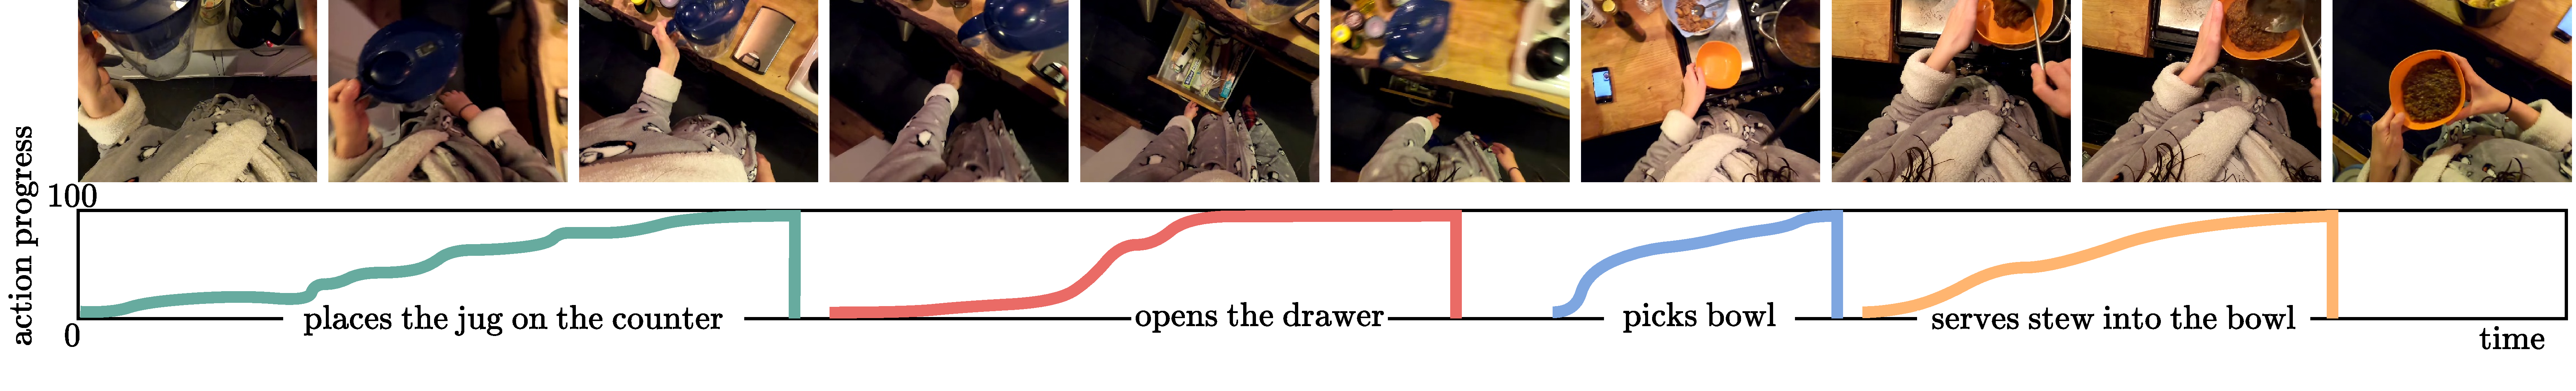
\includegraphics[width=\textwidth]{figs/states/states-action_progress.pdf}
\caption{\textbf{Action Process Prediction (APP)}. Given a video stream of a procedural task, estimate the progress of each ongoing action by inferring the time it will take to complete the action performed. Video sourced from \citep{grauman2024ego} \vspace{1em}}
\label{fig:states::progress}
\end{subfigure}
\begin{minipage}{0.49\textwidth}
\begin{subfigure}{\linewidth}
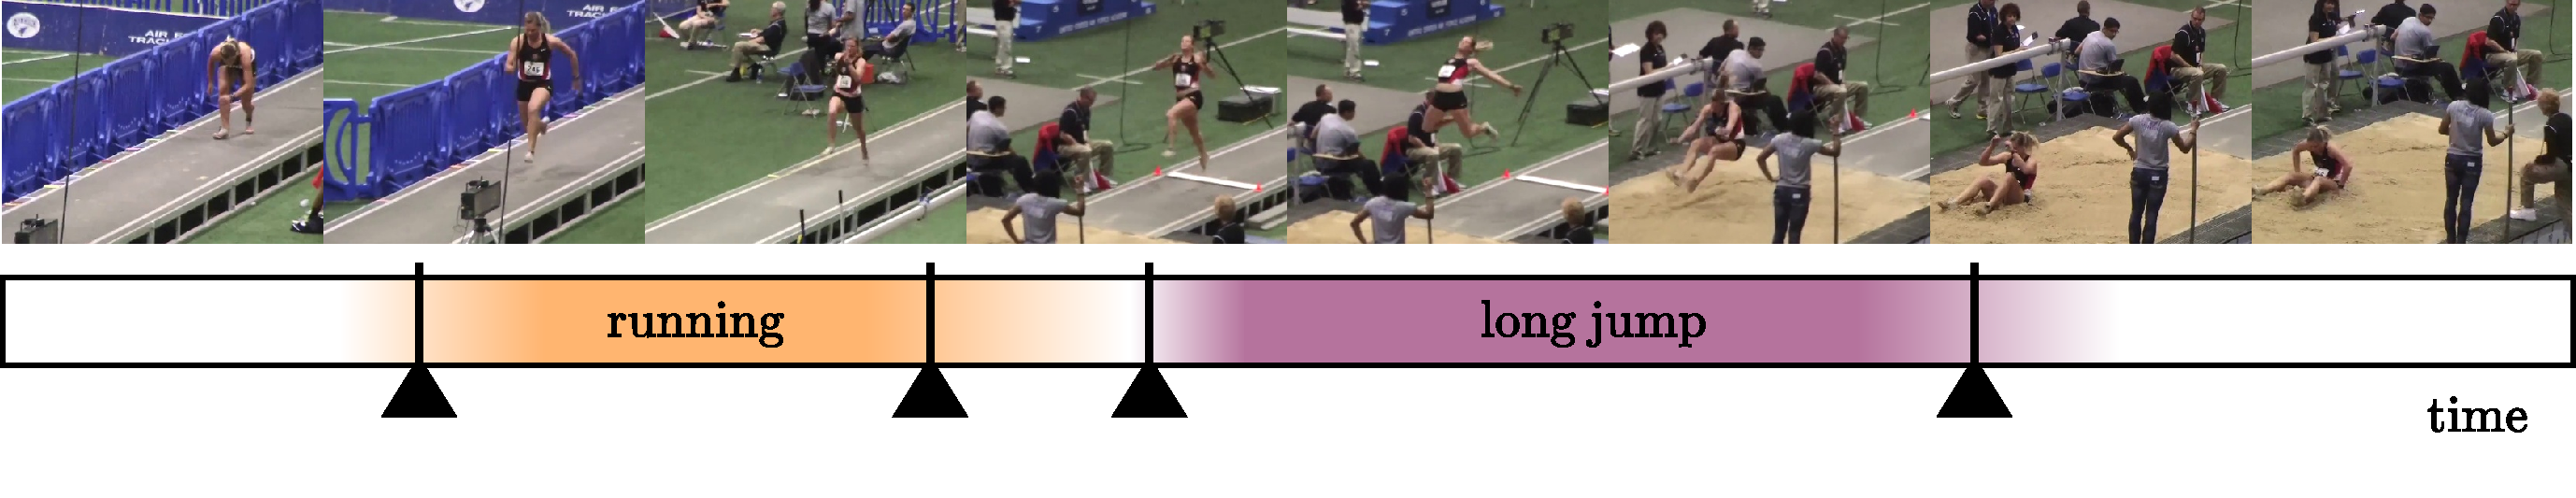
\includegraphics[width=\linewidth]{figs/states/states-event_boundary.pdf}
\caption{\textbf{Event Boundary Detection (EBD)}. Detect the start and end times of ongoing events in video streams. Video sourced from \citep{carreira2017quo} \vspace{1em}}
\label{fig:states::boundary}
\end{subfigure}
\hfill
\addtocounter{subfigure}{1}
\begin{subfigure}{\linewidth}
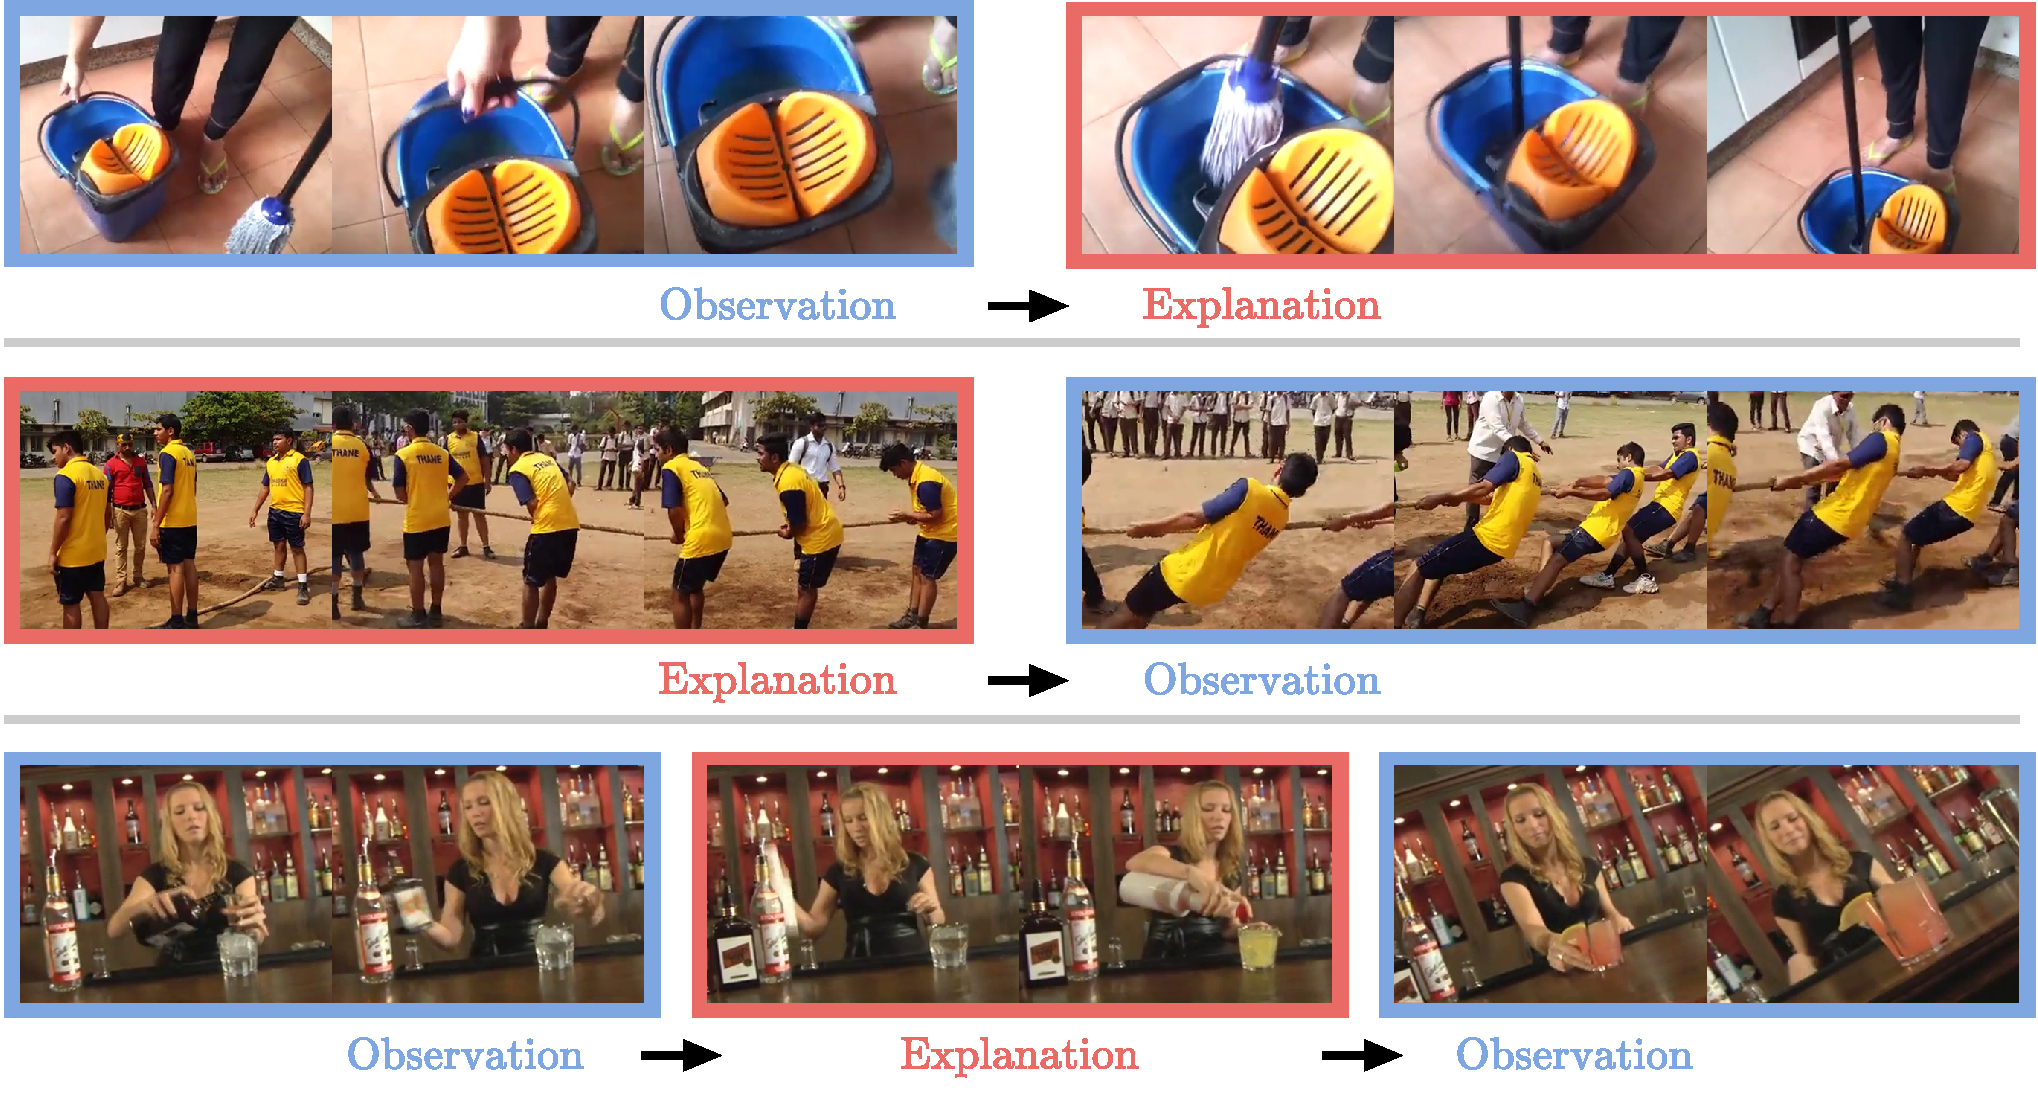
\includegraphics[width=\linewidth]{figs/states/states-abductive reasoning.pdf}
\caption{\textbf{Visual Abductive Reasoning (VAR)}. Given the observable part of the video in \textcolor{babyblue}{blue}. Infer a likely explanation in \textcolor{fadedred}{red} for what follows before, after, or during the observation. The task requires a high-level understanding of the action or activity performed. Video sourced from \citep{liang2022visual} \vspace{1em}}
\label{fig:states::reasoning}
\end{subfigure}
\end{minipage}
\hfill
\begin{minipage}{0.49\textwidth} 
\addtocounter{subfigure}{-1} 
\begin{subfigure}{\linewidth}
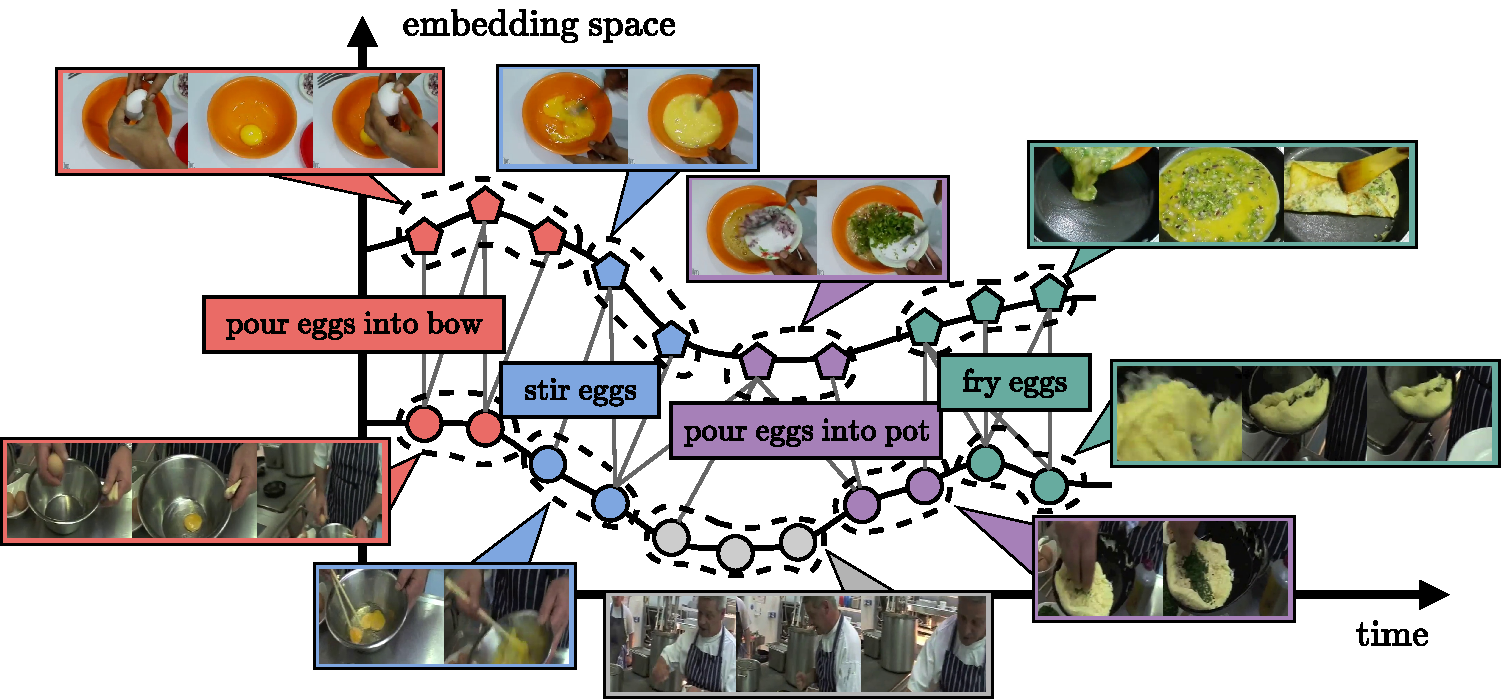
\includegraphics[width=\linewidth]{figs/states/states-alignment.pdf}
\caption{\textbf{Video Alignment (VA)}. Find correspondences across video instances with the same action performed and align them so the execution of the action is synchronized. Video sourced from \citep{tang2019coin} \vspace{.5em}}
\label{fig:states::align}
\end{subfigure}
\hfill
\begin{subfigure}{\linewidth}
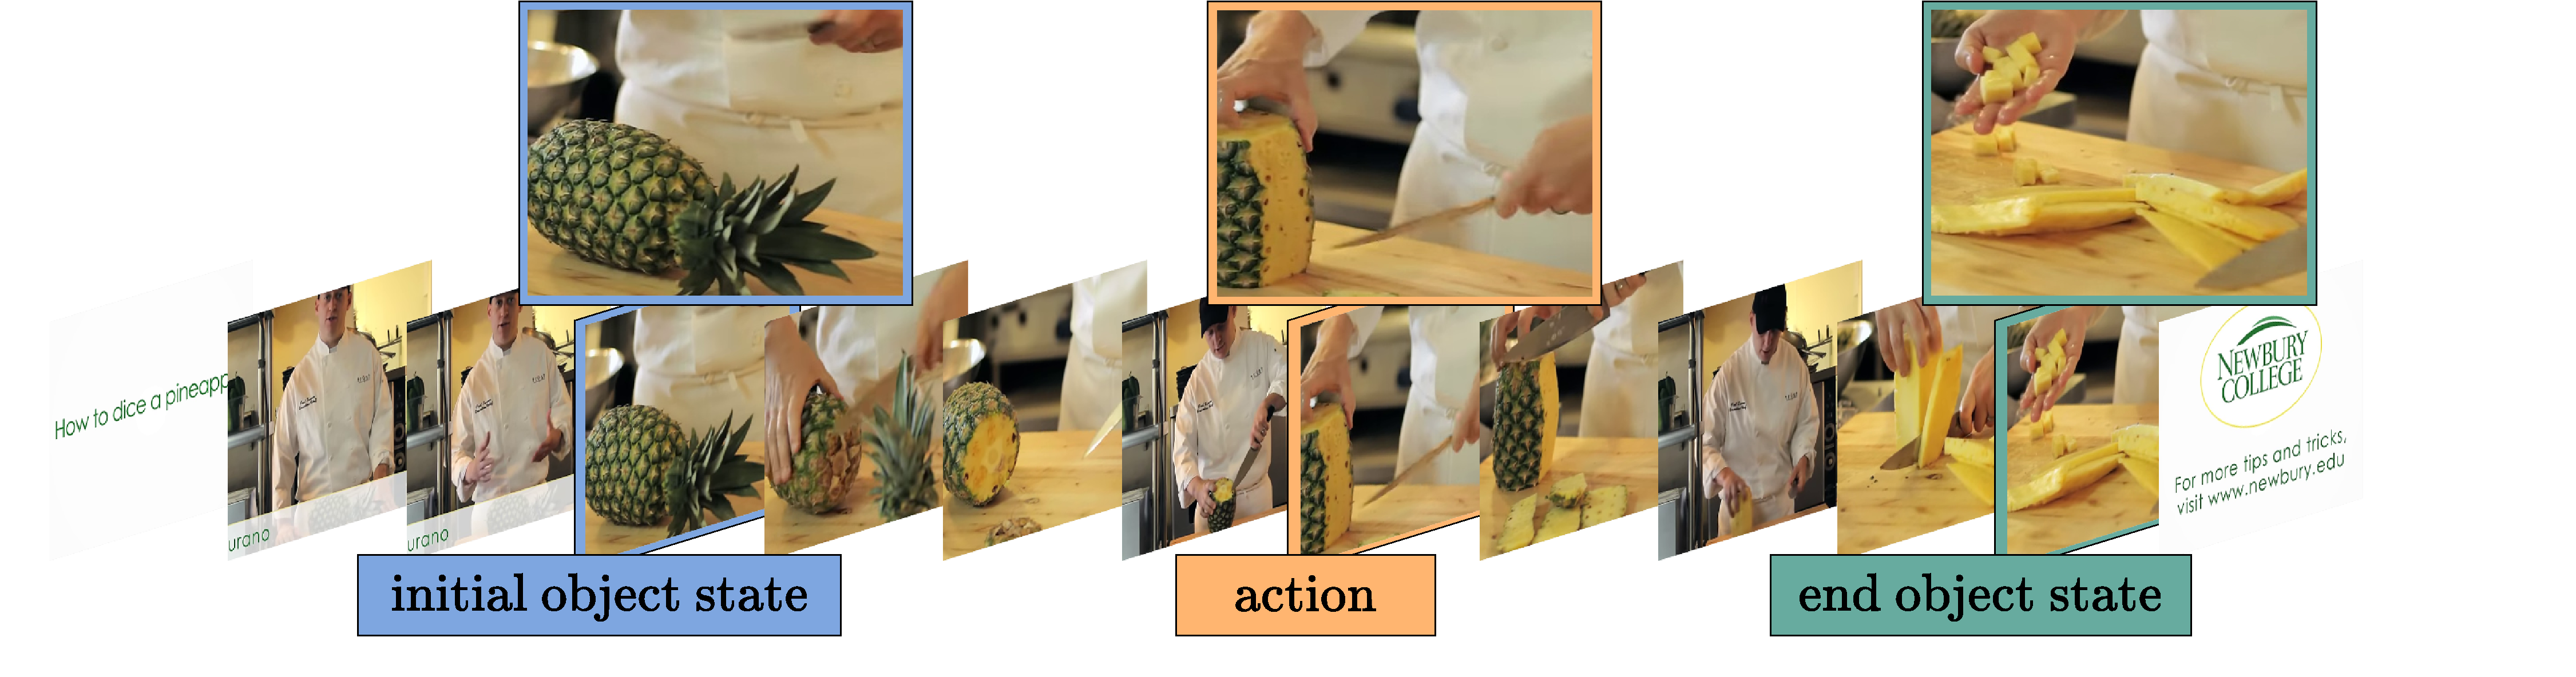
\includegraphics[width=\linewidth]{figs/states/states-object_state_change.pdf}
\caption{\textbf{Object State Change Detection (OSCD)}. State modifying actions such as \textit{cutting}, progressively change the visual appearance of objects from an initial state in \textcolor{babyblue}{blue} to a final post-action execution state in \textcolor{pastelteal}{teal}. OSCD localizes the times that these changes occur. Video sourced from \citep{souvcek2022look}. \vspace{0.5em}}
\end{subfigure}
\end{minipage} % end of second minipage
\begin{subfigure}{\linewidth}
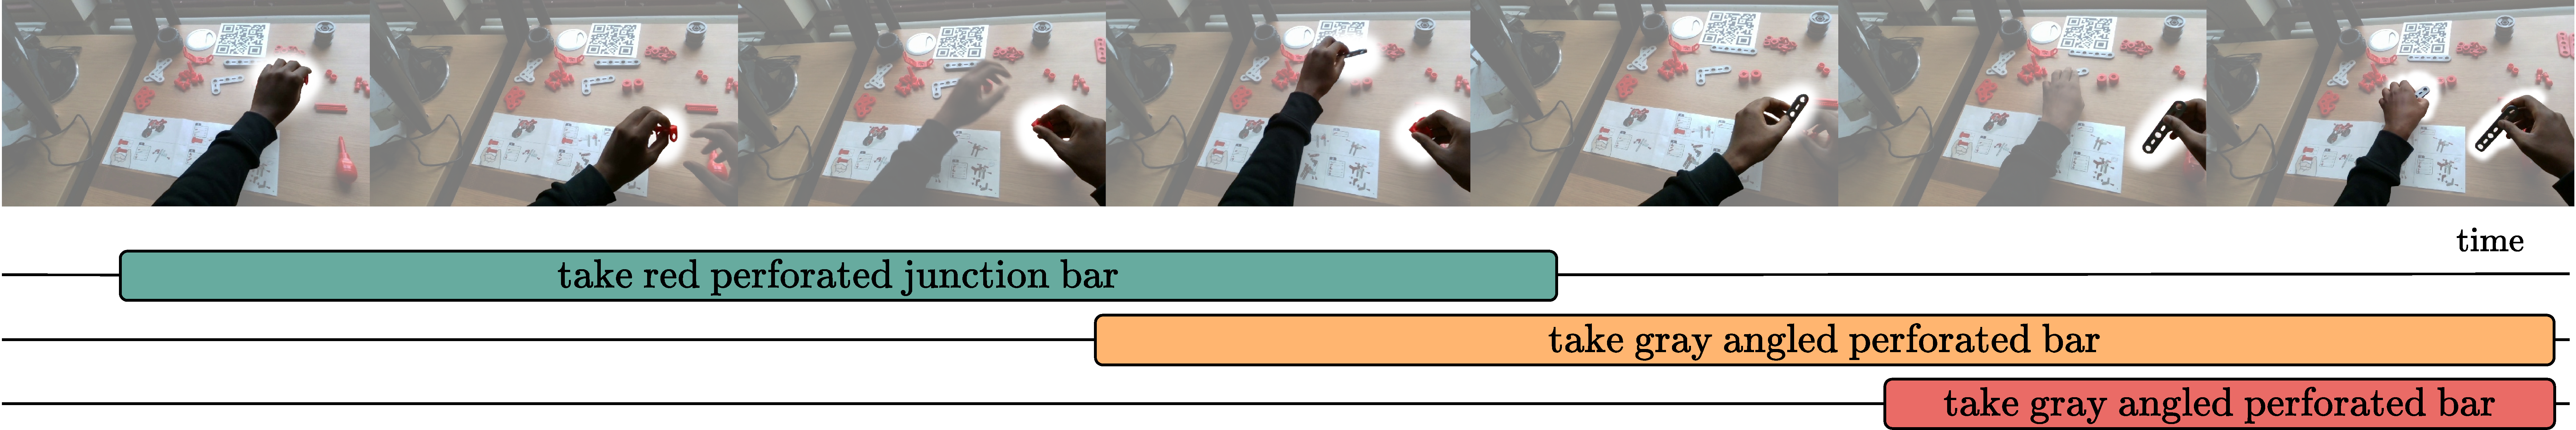
\includegraphics[width=\linewidth]{figs/states/states-active_object.pdf}
\caption{\textbf{Active Object Detection (AOD)}. Given a video in which a person interacts with multiple objects, AOD aims to detect the object the person is currently using. Video sourced from \citep{ragusa2021meccano}.}
\end{subfigure}
\caption{\textbf{Tasks relating to object and action state change}. Each of the presented sets of tasks can involve further specific objectives that correspond and address different aspects.}
\label{fig:state_changes}
\end{figure*}

\subsection{State changes}

Another set of action prediction tasks includes modeling the state changes in the environment, actions, objects, and execution speeds. It can also involve inferring the reasoning for these changes. An overview of the tasks' objectives is visualized in~\Cref{fig:state_changes}.

\noindent
\textbf{Challenges}

% Progress
\noindent
\textbf{Action progress}. Actions can be understood by procedural sets of motions performed towards an intended goal. Vaina and Jaulent \citep{vaina1991object} have suggested that understanding the state and progress of the action at different times can provide a holistic understanding of the intent and objective. In machine vision, an initial approach for Action Progress Prediction (APP)  \citep{fathi2013modeling} used local descriptions to model per-frame state changes. \citep{kataoka2016recognition} used a descriptor to discover transitional actions within activity sequences. \citet{xiong2017pursuit} introduced a score function to distinguish actions based on learned distinctive parts. Becattini \citep{becattini2020done} used actor and scene context information as an additional supervisory signal for APP. \citet{price2022unweavenet} expressed the progress of multiple actions through threads of activities that in long procedural videos can also overlap. Shen and Elhamifar \citep{shen2024progress} causally attended videos to define a task graph for APP over each action. More recently generative approaches \citep{damen2024genhowto} using conditional control \citep{zhang2023adding} and procedural knowledge \citep{ashutosh2024video,zhou2023procedure} have also been used to generate keyframes of changes. 

% Quality and completion
Another line of research works \citep{heidarivincheh2018action,heidarivincheh2016beyond} has also aimed to localize the moments that actions are completed to specific frames. The speed of completion or state changes in actions has also been studied in the context of skill determination \citep{doughty2018s} or their semantic correspondence to textual adverbs \citep{doughty2020action,doughty2022you,moltisanti2023learning}. Scoring approaches \citep{tang2020uncertainty} have been used to study the procedural execution of action in the context of quality assessment. Adjacent tasks such as video captioning and action classification have also been integrated in multi-task settings \citep{parmar2019and}.


\noindent
\textbf{Event boundary detection}. Different from the adjacent well-studied task of action localization, Event Boundary Detection (EBD) \citep{shou2021generic} aims at localizing event changes in videos \emph{regardless of the action classes}.
Aakur and Sarkar \citep{aakur2019perceptual} proposed a self-suprvised objective
in which their model is initially trained to reconstruct subsequently observed features. \citep{shou2021generic} used a self-similarity metric to determine event boundaries by relating encoded frame features. Further EBD approaches \citep{mounir2024streamer} have also studied hierarchies of the video events. 


\noindent
\textbf{Video alignment}. As the performance of individual parts of actions can vary, Video Alignment (VA) methods aim to temporally match key moments in the execution of the same action across videos. Initial efforts, motivated by temporal coherence \citep{goroshin2015unsupervised,fernando2017self,zhang2023modeling}, have studied VA through approaches based on Canonical Correlation Analysis (CCA) \citep{andrew2013deep} or contrastively creating joint representations from multiple viewpoints \citep{sermanet2018time}. Dynamic Time Wraping \citep{sakoe1978dynamic} is an algorithm that aligns variable length signals which has also been adopted for VA \citep{chang2019d3tw,hadji2021representation,dvornik2021drop}. A more recent self-supervision objective \citep{dwibedi2018temporal} for VA is to train a video model to project per-frame embeddings in pairs of target videos by matching embeddings of one video to the nearest neighbor embeddings of the other. This approach was extended in subsequent works by including context from the entire video \citep{haresh2021learning}, creating anchor frames to align redundant frames \citep{liu2022learning}, leveraging embeddings from text \citep{epstein2021learning}, and regularizing the correspondence to repetitions of the same action \citep{donahue2024learning}.
 

\noindent
\textbf{Abductive reasoning}. A key element in action understanding is the intended goal. High-level reasoning of events has initially been considered in hierarchies with approaches using rule-based \citep{hakeem2004ontology} or conditionality of action occurrence \citep{albanese2010pads} at each hierarchy. \citet{pei2011parsing} detected atomic actions with graph representations to decompose complex events. Visual Abductive Reasoning (VAR) \citep{liang2022visual} is the vision-language task that uses characteristics of partial observations as a premise and requires formulating an explanation. VAR Models have been based on modeling intention with contrastively learning visual and language context \citep{li2023intentqa}, modeling timelines for news story understanding \citep{liu2023video}, or forecasting actions with multi-modal inputs \citep{zhu2023personality}. Evaluation of VAR models has also been studied in counterfactual vision-language pairs \citep{park2022exposing} similar to text-only tasks \citep{ippolito2019unsupervised,huang2020inset}.

\noindent
\textbf{Object state change}. Actions such as `whisking eggs', `filling cup', or `assembling legos' can often alter the appearance or state of objects. Object State Change Detection (OSCD) approaches associate the visual changes with changes in the states of objects in the scene. Efforts \citep{alayrac2017joint,liu2017jointly,zhuo2019explainable} have initially focused on state modifications that do not involve significant appearance changes, e.g; `open/close door' or `fill/empty cup'. \citet{hong2021transformation} proposed a reasoning-based approach defining a triplet of complexities for single- and multi-step transformations and multi-step transformations with additional viewpoint changes. Other reasoning-based approaches include the use of language \citep{xue2024learning} and visual exemplars of start and end states \citep{souvcek2022look}. OSCD has also been studied in combination with other tasks including cross-state object segmentation \citep{yu2023video}, cross-action relevance \citep{alayrac2024multi}, or inspired by state-disentanglement for images \citep{gouidis2023leveraging,nagarajan2018attributes,saini2022disentangling}, generating start and end states by given context and scene prompts \citep{saini2023chop}.



\noindent
\textbf{Active object}. Actions can include multiple objects during their execution. Active Object Detection (AOD) specifies the objects relevant to the currently performed atomic action. This task has recently gained interest as scenes can often be cluttered \citep{ragusa2021meccano} or a varying number of objects can be used for a single action \citep{miech2019howto100m}. \citet{nagarajan2019grounded} specifically focused on localizing the human-object interaction areas to define focal points of importance during the execution of actions. \citep{fu2021sequential} defined a voting module over potential bounding boxes corresponding to the active object. \citet{kim2021hotr} used a parallelized model for separately detecting instances and in turn detecting hand-object interaction. Yang and Liu \citep{yang2024active} used scene context from text to define plausible interactions with target objects for AOD.  


\noindent
\textbf{Future outlooks}.



\subsection{Anomaly detection}

\noindent
\textbf{Close-set}. Anomalies can be discovered by \emph{close-set} tasks that aim to model both normal and abnormal sequences. \citet{sultani2018real} used Multiple Instance Ranking (MIL) \citep{dietterich1997solving} to define positive groups that include videos with at least a single abnormal segment and negative groups of normal videos. The objective in turn compared the maximum anomaly score between the assigned positive and negative groups. Subsequent efforts \citep{dubey20193d,zhang2019temporal,zhu2019motion,feng2021mist,tian2021weakly,almarri2024multi} have built upon MIL with learned features \citep{dubey20193d}, or pseudo labels \citep{feng2021mist}. With MIL being influenced by the dominant negative instances, \citep{zhang2019temporal} proposed inner-group sampling, \citep{pu2023learning,zhu2019motion} used temporal weighting, and \citep{tian2021weakly} aim to maximize the separability between normal and anomalous representations. The use of multiple temporal pretext tasks \citep{almarri2024multi,georgescu2021anomaly} and temporal scales \citep{li2022scale} has also been explored. \citep{chen2023mgfn} used a contrastive objective between representations of normal and abnormal videos. Clustering approaches focus on sparsity modeling \citep{lu2013abnormal}, enforcing high distribution variance in abnormalities \citep{li2021deep}, combining dense/spare clusters for normal/abnormal segments \citep{zaheer2020claws}, and using pseudo labels for anomalous segements \citep{zaheer2020self}. Another set of methods \citep{zhong2019graph,purwanto2021dance} has included graph networks to sequentially detect abnormal segments. More recent methods have distinguished between states with the use of additional modalities such as audio \citep{wu2020not} and language context \citep{yang2024text,zanella2024harnessing}.


\begin{figure*}[!ht]
    \centering
    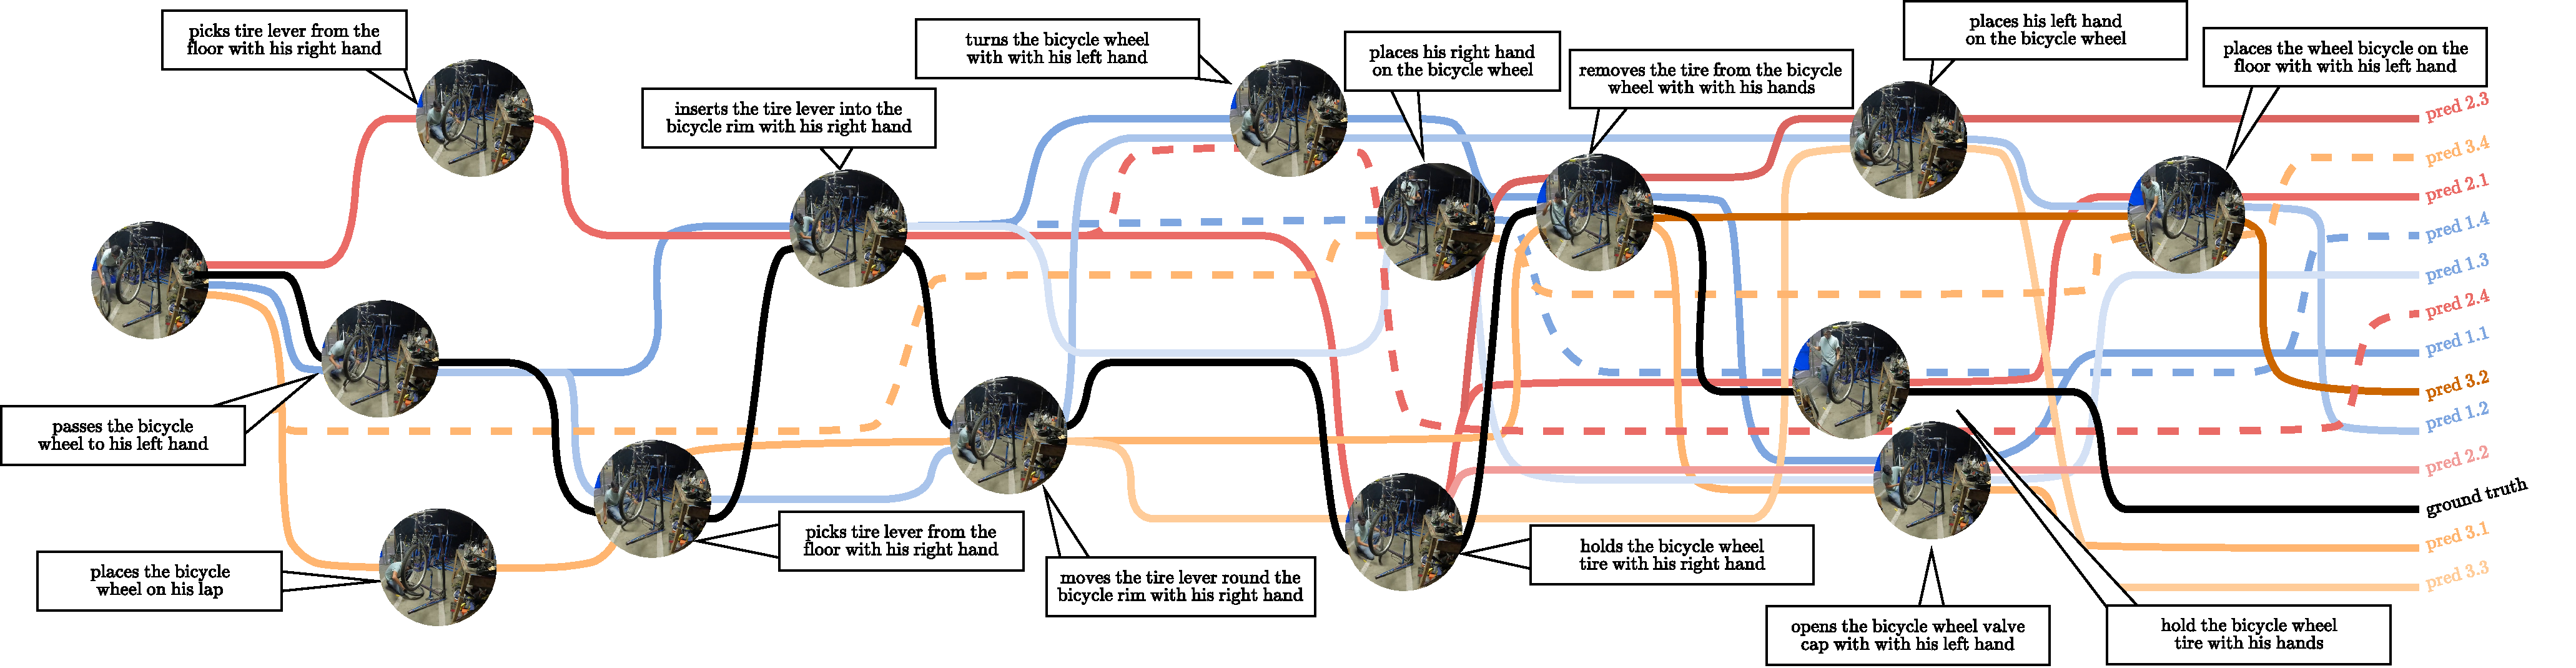
\includegraphics[width=\linewidth,trim={0cm 0 0cm 0},clip]{figs/narrative_chart_ego_exo.pdf}
    \caption{\textbf{Visualization of forecasted future actions}. Starting from the observed action, anticipation approaches infer the sequence of probable next actions. Increases in the number of future actions to anticipate also relate to the number of possible scenarios. Predictions are shown in a narrative chart format similar to \citep{randal2009movie}.
    Example selected from \citep{grauman2024ego}.} 
    \label{fig:narration_chart}
\end{figure*}

\noindent
\textbf{Open-set}. As the close-set solutions can only model abnormalities in labeled data, models cannot effectively generalize to distributions different than those they are trained in. This has been studied by \citet{zhao2011online} and later \citet{luo2017revisit} as a sparse-coding \citep{lee2006efficient} problem in which the model is trained to reconstruct normal sequences. Abnormalities can then be inferred through the reconstruction loss. Temporal regularity can also be modeled with autoencoders as a reconstruction task \citep{hasan2016learning}. Further AE-based approaches also used pseudo representations to improve abnormal sequence scarcity in the embedding space \citep{astrid2021synthetic,astrid2021learning} or used prototypes of normal sequences \citep{park2020learning}. Other works have constrained the representation space of normal sequence through optimizing piecewise linear decision boundaries \citep{wang2019gods}. Two-steam AE frameworks \citep{cho2022unsupervised,nguyen2019anomaly} have also been used to separately reconstruct appearance and motion characteristics of normal sequences. Generative approaches \citep{micorek2024mulde} have also focused on the latent space with Gaussian mixture model and inferred an anomaly score across all noise levels.

As part of the video anomaly detection requires 
\citep{fioresi2023ted}

trajectory-based video anomaly detection methods
\citep{markovitz2020graph,morais2019learning,flaborea2023multimodal,stergiou2024holistic}.


%\subsection{Online clustering}


\section{Future forecasting}
\label{sec:forecasting}


\subsection{Action anticipation}


Action Anticipation (AA) requires recognizing current action(s) performed at $\tau_1$ to forecast a \emph{proceeding action} $\tau_2$. In contrast to the partial observations for EAP, anticipation tasks only rely on the expected sequence with which actions can be performed. Early works \citep{kitani2012activity,kuehne2014language,koppula2015anticipating} have used graphs to model this sequentiality of actions over time. However, given the limited long-range dependency of graph-based approaches, works have explored either the progress in the execution of actions \citep{abu2018will,furnari2019would,ke2019time}, the motion transition intensity between actions \citep{huang2014action}, gaze and hand information \citep{shen2018egocentric}, or used future-action objective with multiple predictions \citep{furnari2018leveraging,zatsarynna2024gated}. Despite the diversity of the approaches, some challenges remain present throughout the proposed methods.

\noindent
\textbf{Challenges}


\noindent
\textbf{Embedding similarity maximization}. The representations of future actions can be used as a target for learned embeddings. A large number of methods in the literature have thus used future embedding reconstruction tasks to in turn infer future action labels. \citet{gao2017red} used a recurrent decoder to regress future embeddings with an additional policy for class predictions over time. Interaction between objects and actors \citep{sun2019relational,luc2018predicting} has also been explored by early attempts. 
Subsequent methods aimed to either maximize the similarity between future and current embeddings through memory banks \citep{liu2022hybrid},
optimize latents representing intended goals \citep{roy2022action}, prototypes \citep{diko2024semantically}, or adversarial representations \citep{gammulle2019predicting}. Other generative approaches use pose information as priors \citep{villegas2017learning} or focus on the extrapolation of activity trajectories \citep{chi2023adamsformer}.
Autoregressive approaches have recently shown great promise using either contrastive objectives \citep{wu2020learning}, causal attention \citep{girdhar2021anticipative}, or audio-visual inputs \citep{zhong2023anticipative}. As future predictions depend on the usefulness of current observations, works have also integrated uncertainty terms in their predictions. \citet{vondrick2016anticipating} regressed towards multiple plausible future embeddings, \citet{abdelsalam2023gepsan} grounding the sequentiality of visual embeddings to language, while \citet{guo2024uncertainty} defined probabilistic transformer outputs through a top-k prediction loss similar to \citep{furnari2018leveraging}.

\noindent
\textbf{Long-term anticipation}. The anticipation of the future can also be extended to forecasting multiple upcoming actions over a longer temporal duration. \citet{bokhari2017long} used a q-learning framework with reward functions for the activity label, and locations where actions are performed. \citet{nawhal2022rethinking} used a two-stage approach to first infer potential labels and use their logits alongside visual features to predict future action segments. Similarly, \citet{gong2022future} used learnable latents for the future embeddings and cross-attend \citep{jaegle2021perceiver,lee2019set} them with observed video embeddings. Generative approaches have learned future embeddings based on pre-defined temporal states \citep{piergiovanni2020adversarial}, logit sequences \citep{zhao2020diverse}, using cyclic consistency \citep{abu2021long}, or through learning the expected variance in future representations \citep{mascaro2023intention,patsch2024long}. Recently, \citet{mittal2024can} used general language and visual queries to infer prediction through LLMs.

\noindent
\textbf{Next active object}. A recently introduced set of anticipation tasks also study object-centric future forecasting. Next active object anticipation aims to forecast the objects that will be used in future actions with approaches using predictions on the salient regions \citep{dessalene2021forecasting}, hand position generated representations \citep{jiang2021predicting}, or autoregressively attending object and visual information \citep{thakur2024anticipating}. Other methods may also forecast human object interaction regions \citep{liu2020forecasting,liu2022joint,roy2024interaction}, object relations \citep{roy2021action,zatsarynna2021multi}, or time-to-contact estimates \citep{mur2024aff}.

\noindent
\textbf{Future outlooks}.


\begin{figure}[t]
    \centering
    \includegraphics[width=\linewidth,height=3cm]{example-image-c}
    \caption{\textcolor{red}{TODO: Visual examples of generative models.}}
\end{figure}


\subsection{Video Generation \ding{52}}

\noindent
\textbf{Generative models}
short sequences GANs
\citep{clark2019adversarial}
\citep{saito2017temporal}
\citep{luc2020transformation}
\citep{vondrick2016generating}
\citep{menapace2021playable}
\citep{yu2022generating}

GANs for long sequences
\citep{ge2022long}
\citep{brooks2022generating}
\citep{shen2023mostgan}
\citep{skorokhodov2022stylegan}

Attention-based generative models
\citep{han2022show}
\citep{hu2022make}

\noindent
Diffusion
\citep{ge2022long}
\citep{blattmann2023align}
\citep{nikankin2023sinfusion}
\citep{yang2023video}
\citep{ho2022video}
\citep{he2022latent}
\citep{wu2023tune}
\citep{harvey2022flexible}
\citep{yugenerating}
\citep{liu2024sora}
\citep{hong2022cogvideo}
\citep{yu2023avideo}
\citep{zeng2024make}
\citep{yu2024efficient}

\noindent
\textbf{Text-conditioned diffusion}
\citep{yan2021videogpt}
\citep{gupta2023photorealistic}
\citep{zhuang2024vlogger}

\noindent
\textbf{Future generation with diffusion}
\citep{fu2023tell}

autoregressive \citep{ho2022imagen}
\citep{villegas2022phenaki}
\citep{singer2023make}
\citep{wu2021godiva}
\citep{wu2022nuwa}


\citep{chang2024look}

\section{Challenges and peeking through the future}
\label{sec:outlook}

\section{Discussion}
\label{sec:discussion}

{
\bibliography{egbib}
}

%\begin{IEEEbiographynophoto}{Jane Doe}
%Biography text here without a photo.
%\end{IEEEbiographynophoto}

%\begin{IEEEbiography}[{\includegraphics[width=1in,height=1.25in,clip,keepaspectratio]{fig1.png}}]{IEEE Publications Technology Team}
%In this paragraph you can place your educational, professional background and research and other interests.\end{IEEEbiography}

\end{document}
\endinput
%%
%% End of file `elsarticle-template-num.tex'.
